\documentclass[../main.tex]{subfiles}

\begin{document}

\renewcommand{\labelitemi}{\ding{226}}
\renewcommand{\labelitemii}{\ding{227}}

\part{Heavy neutrino study}

\chapter{Prospects in T2K}


In the current work we study a possibility of the improvement of the constraints on the mixing elements of the HNL in the T2K experiment. The details about the experimental setup are described~in~the~\autoref{part:T2K:general}. The main feature of the experiment for the HNL search is very intensive proton beam providing by J-PARC accelerator. The beam operation is overviewed~in~the~\autoref{ch:T2K:nu_beam}. The focusing system allow to perform the analysis focusing positive or negative mesons from the proton interactions. As mentioned in the \nameref{ch:intro:HNL}, heavy neutrinos could be produced in the mesons decays. As a result there are two possible strategies of the HNL search:
\begin{itemize}
    \item measurement of the meson decay kinematics. The effect is proportional to $\left|U_l\right|^2$;
    \item search for decay products of the heavy neutrino. As both HNL production and decay are proportional to $\left|U_l\right|^2$, the final effect $\propto\left|U_l\right|^4$.
\end{itemize}

The schema of the T2K experiment is shown in~\autoref{fig:HNL:t2k_schema}. The muon monitor is the only instrument that could measure the muons directly from the meson decay. In spite of its extreme usefulness for the neutrino beam intensity and direction measurements, it could not provide necessary precision for the search of the HNL through the detection of the muons from the meson decay. Thus the only way of the heavy neutrino study in the T2K is search for the HNL decays in the near detector complex. The near detector complex (\autoref{ch:T2K:nd}) consists of on-axis INGRID detector and off-axis ND280. The most precise analysis could be done with the the ND280's time projections chambers. As we are looking for the HNL decays in the neutrino beam the gaseous detectors will observe much less background from the neutrino interactions comparing to scintillators. There are phenomenological studies~\cite{Asaka2012} that indicate the prospects of such analysis in the T2K experiment.

\begin{figure}[!ht]
    \centering
    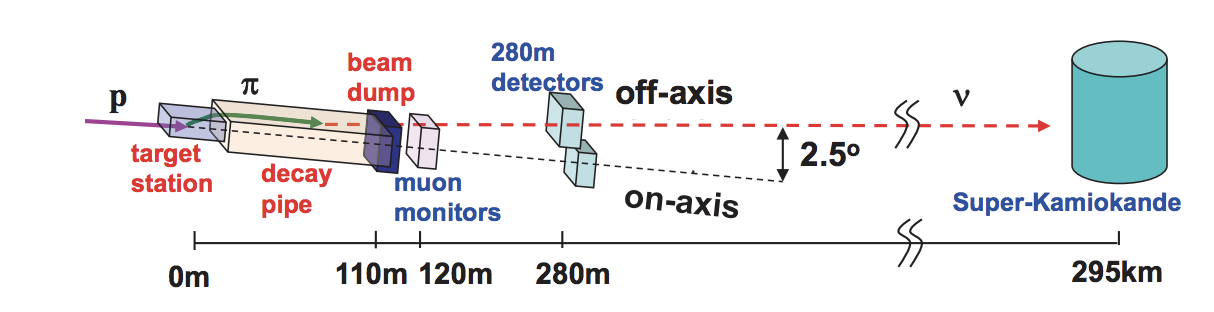
\includegraphics[width=\linewidth]{t2k_schema.png}
    \caption{A schematic view of the neutrino beamline and the detectors in the T2K experiment.}
    \label{fig:HNL:t2k_schema}
\end{figure}

With the 30 $GeV$ proton beam mainly pions are produced with some fractions of kaons. The comparison of the neutrino flux from different parent particles are presented~in~\autoref{fig:HNL:meson_flux}. As we want to study the maximum range of the HNL mass we will concentrate on the kaon decays. Thus we will be able to study the mass region up to 493 $MeV/c^2$. The overview of the HNL nature including the relation with the Standard Model particles is presented~in~\autoref{ch:intro:HNL}. The particular production and decay modes of the heavy neutrino masses that are available for the analysis in our experiment are summarized in the kinematic scheme in~\autoref{fig:HNL:mass_scale} with specific HNL mass region for each of them.

\begin{figure}[!ht]
    \centering
    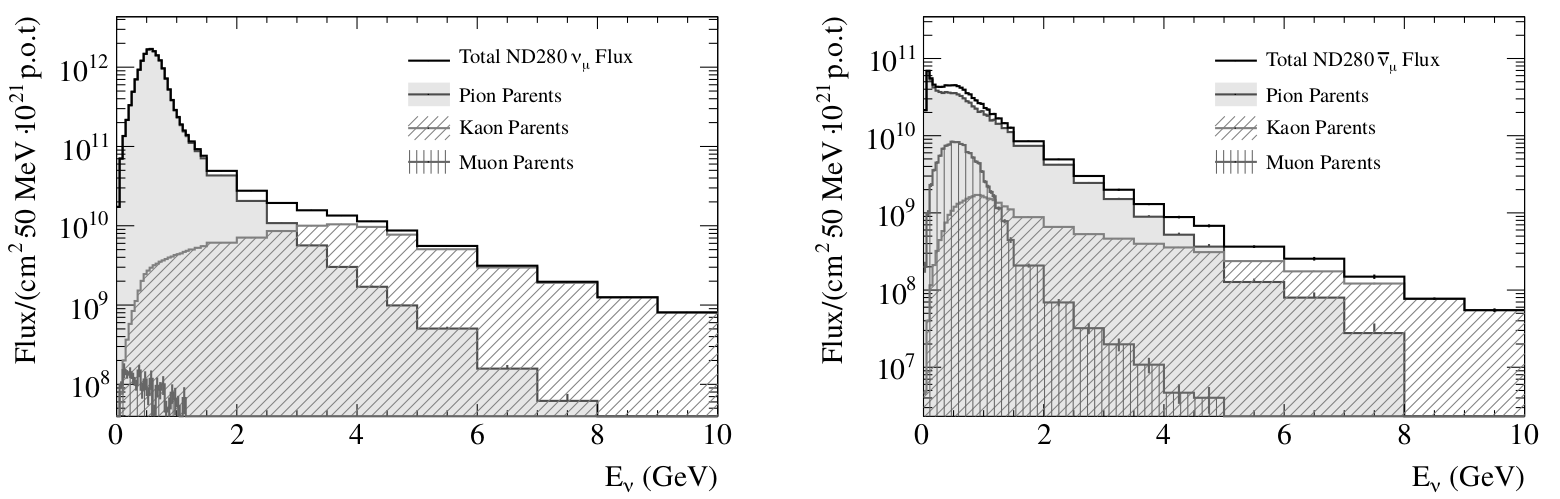
\includegraphics[width=\linewidth]{meson_flux}
    \caption{The muon neutrino and anti-neutrino flux prediction at the ND280 broken down by the neutrino parent particle type.}
    \label{fig:HNL:meson_flux}
\end{figure}

\begin{figure}[!ht]
    \centering
    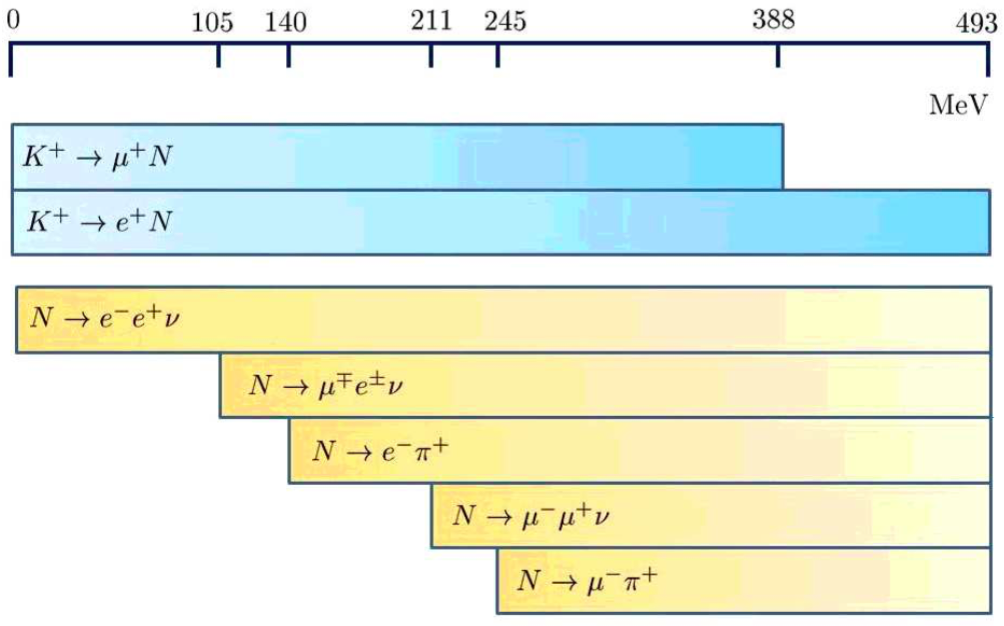
\includegraphics[width=0.7\linewidth]{HNL_mass_scale}
    \caption{Summary of the production and detection processes of the heavy neutrino available for the analysis with the ND280. The horizontal axis corresponds to the HNL mass}
    \label{fig:HNL:mass_scale}
\end{figure}

As one can see from the scheme in our study we will concentrate on the two and tree body decays of the heavy neutrino.

\begin{eqnarray}
    &N\to\ell^{\pm}\pi^{\mp} &\\
    &N\to\ell^{\pm}\ell^{\mp}\nu & \\
\end{eqnarray}

We would like to highlight the importance of the study of a HNL dimuon decay mode: $N\to\mu\mu\nu$. This decay has charge and neutral current contributions shown in Fig.~\ref{fig:DimuonFeynman} (from~\cite{Johnson1997}).

\begin{figure}[!ht]
    \begin{minipage}[!ht]{0.49\linewidth}
        \center{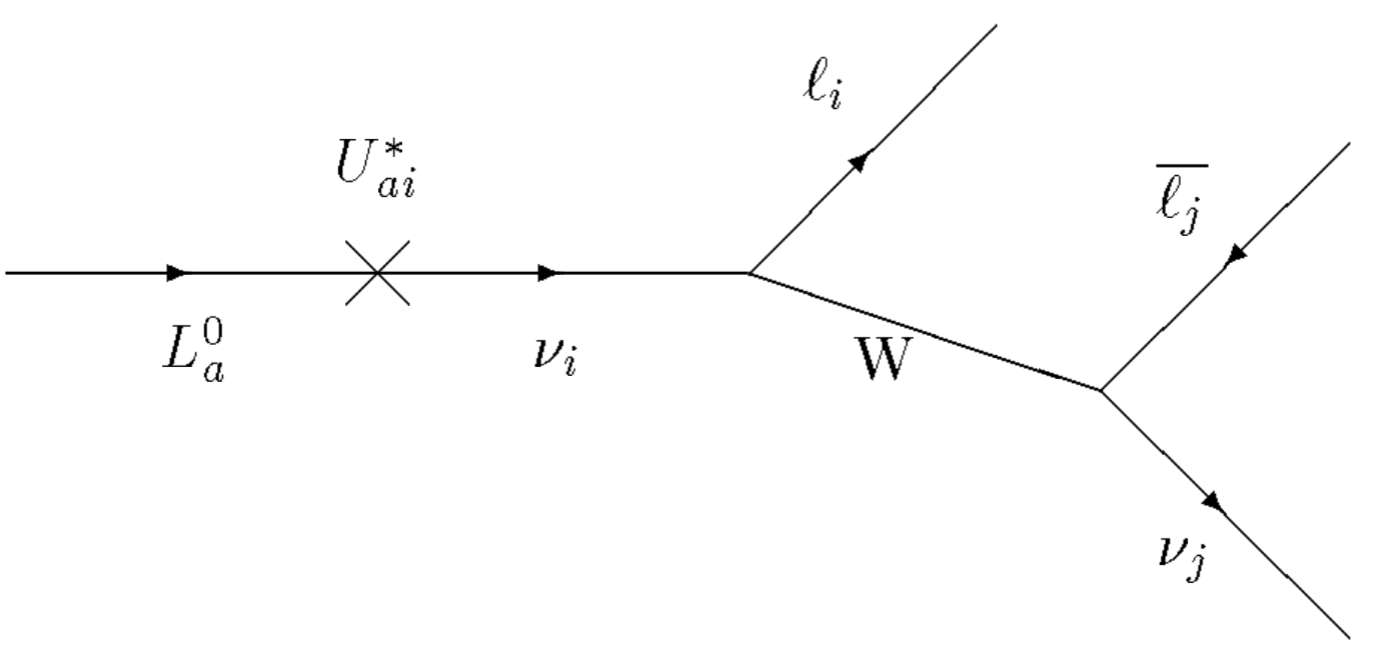
\includegraphics[width=\linewidth]{DiMuonCC.png} \\ a) }
    \end{minipage}
    \hfill
    \begin{minipage}[!ht]{0.49\linewidth}
        \center{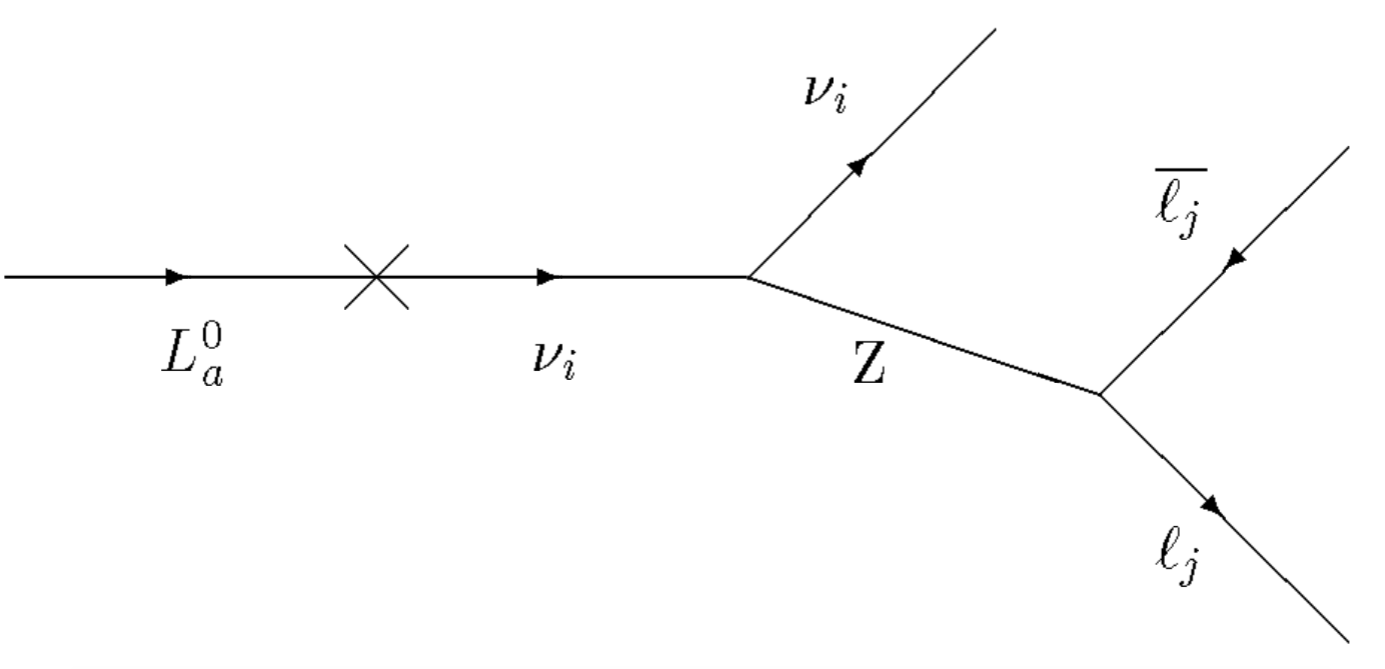
\includegraphics[width=\linewidth]{DiMuonNC.png} \\ b)}
    \end{minipage}
    \caption{Feynman diagrams for the HNL decay $N\to\mu\mu\nu$ via charged (a) and neutral (b) current.}
    \label{fig:DimuonFeynman}
\end{figure}

If the HNL decays via NC, any type of the active neutrino could be produced ($\nu_{e}, \nu_{\mu}, \nu_{\tau}$), so we can study the mixing element including $|U\tau|$. This is interesting as the upper limits on this element are rather high.

\todo{reference to the figure in intro}.

The T2K experiment uses neutrino beam from $\pi^\pm$ and $K^\pm$ decays. In our study a search of HNL from both $K^+$ and $K^-$ decays is carried out in order to increase sensitivity because of the larger statistics. We assume the Majorana nature of a HNL, this allows to study decays of $K^+$, $K^-$ and both decay modes of a heavy neutrino to $\ell^{\pm}\pi^{\mp}$.

As we focus on search of the HNL decay there are two analysis methods:
\begin{itemize}
  \item search for a peak in the HNL candidate invariant mass spectrum
  \item search for a rare event in a low background environment
\end{itemize}

The first one requires applying some simple cuts and then study difference between data and MC estimation with a peak shape. We need a rather accurate background prediction for this method. Also invariant mass resolution is one of the most important issue. We have studied the possible resolution for the HNL signal samples. The events that pass all the cuts described in the~\autoref{sec:HNL:sel} give as the reconstructed mass distribution. The examples of such distribution are presented in~\autoref{fig:HNL:InvMass}. The resolution of the invariant mass reconstruction on the HNL mass is shown in~\autoref{fig:HNL:InvMassPlot}. As one can see, RMS is quite large $\approx70MeV$. The main background processes for the HNL decay are  interactions of the active neutrinos. In near detector there are three TPCs filled with argon gas. The cross sections of the neutrino interactions in gas are not studied well. Studies of these events were performed by ArgoNeuT group~\cite{Acciarri2014}. In our momentum region ($\approx1GeV$) the uncertainties are relatively large. Other background processes can be $K^0, \Lambda, \eta$ decays, deep inelastic neutrino scattering, etc. (\autoref{sec:HNL:bg}) that are also poorly studied. Because of this we can not provide needed accuracy of the background prediction and the method of the invariant mass peak search can not be applied.
\begin{figure}[!ht]
    \begin{minipage}[!ht]{0.49\linewidth}
        \center{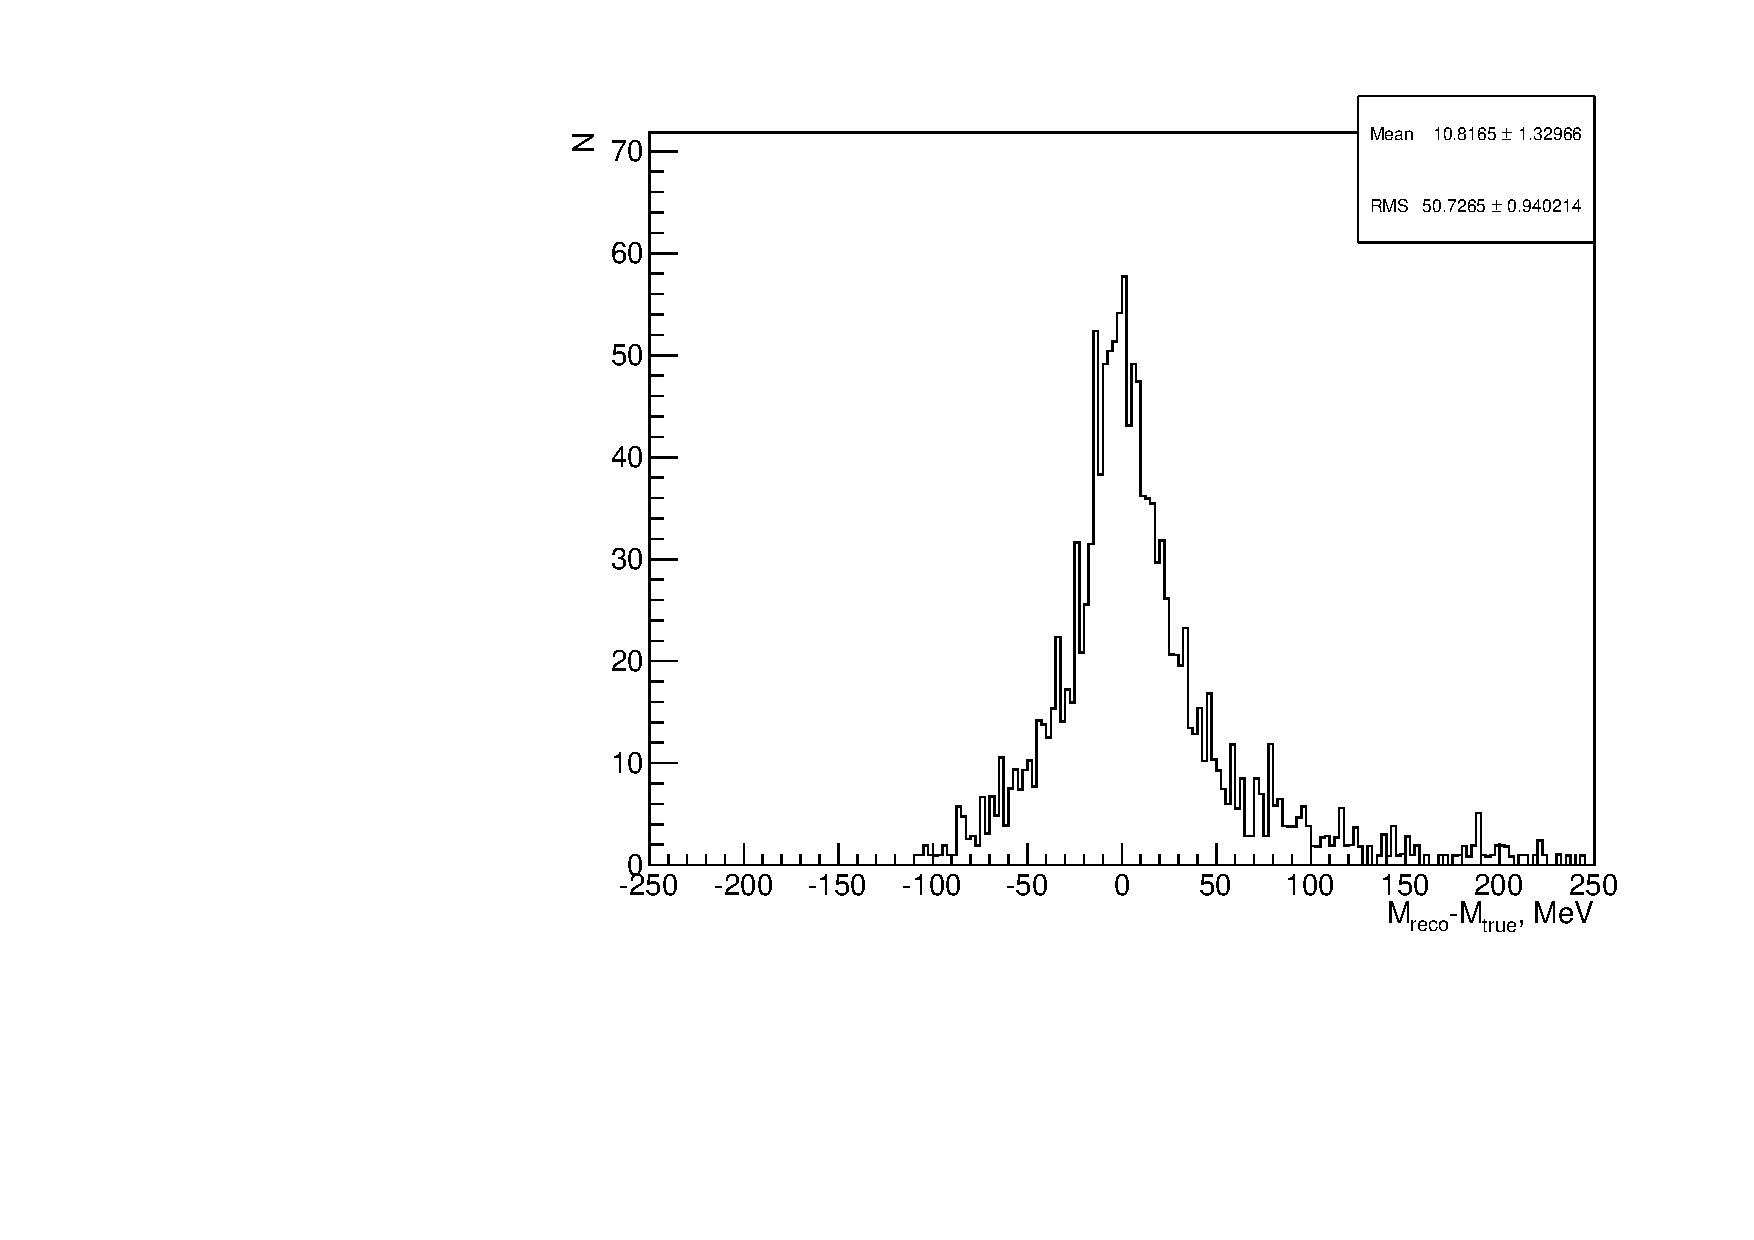
\includegraphics[width=\linewidth]{InvMass036}}
    \end{minipage}
    \hfill
    \begin{minipage}[!ht]{0.49\linewidth}
        \center{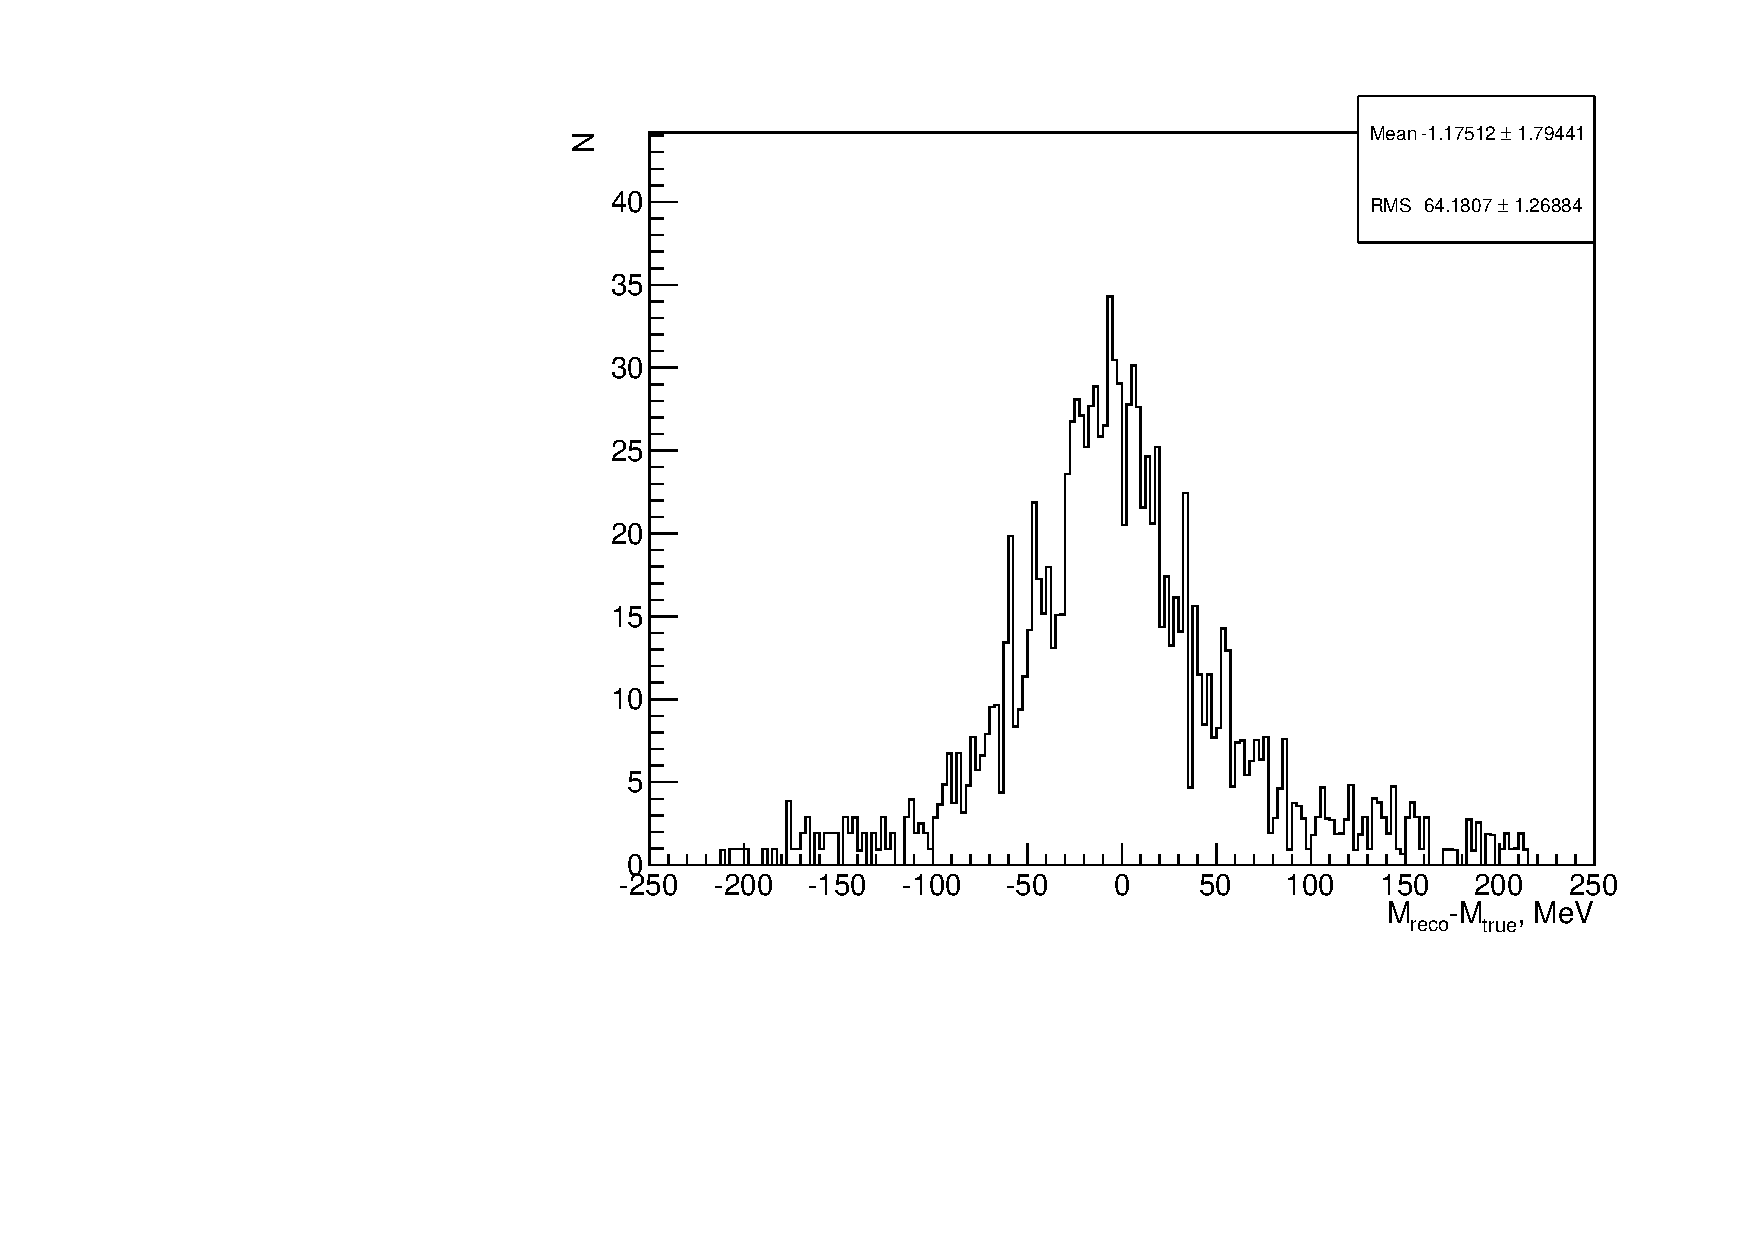
\includegraphics[width=\linewidth]{InvMass048}}
    \end{minipage}
    \caption{HNL invariant mass resolution. Left is for $M_{HNL}=360$ MeV, right is for $M_{HNL}=480$ MeV for the $\mu\pi$ mode.}
    \label{fig:HNL:InvMass}
\end{figure}

\begin{figure}[!ht]
    \begin{minipage}[!ht]{0.49\linewidth}
        \center{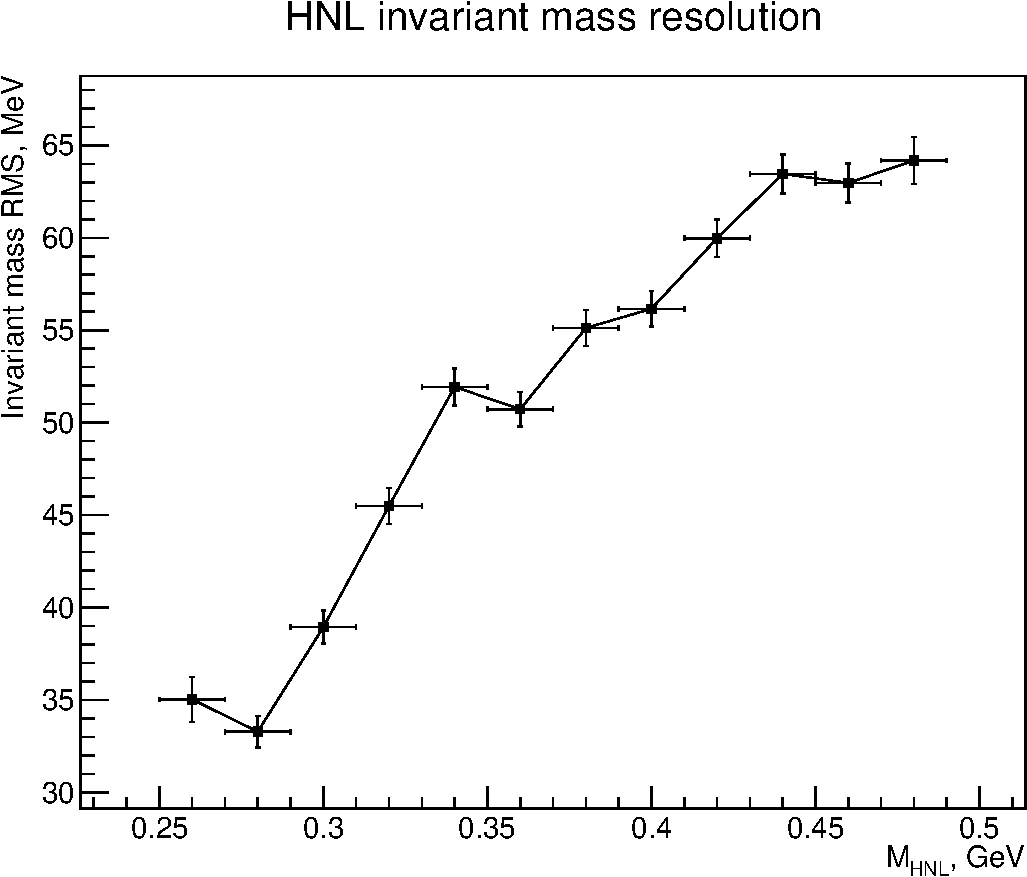
\includegraphics[width=\linewidth]{InvMassMuPlot} \\ a)}
    \end{minipage}
    \hfill
    \begin{minipage}[!ht]{0.49\linewidth}
        \center{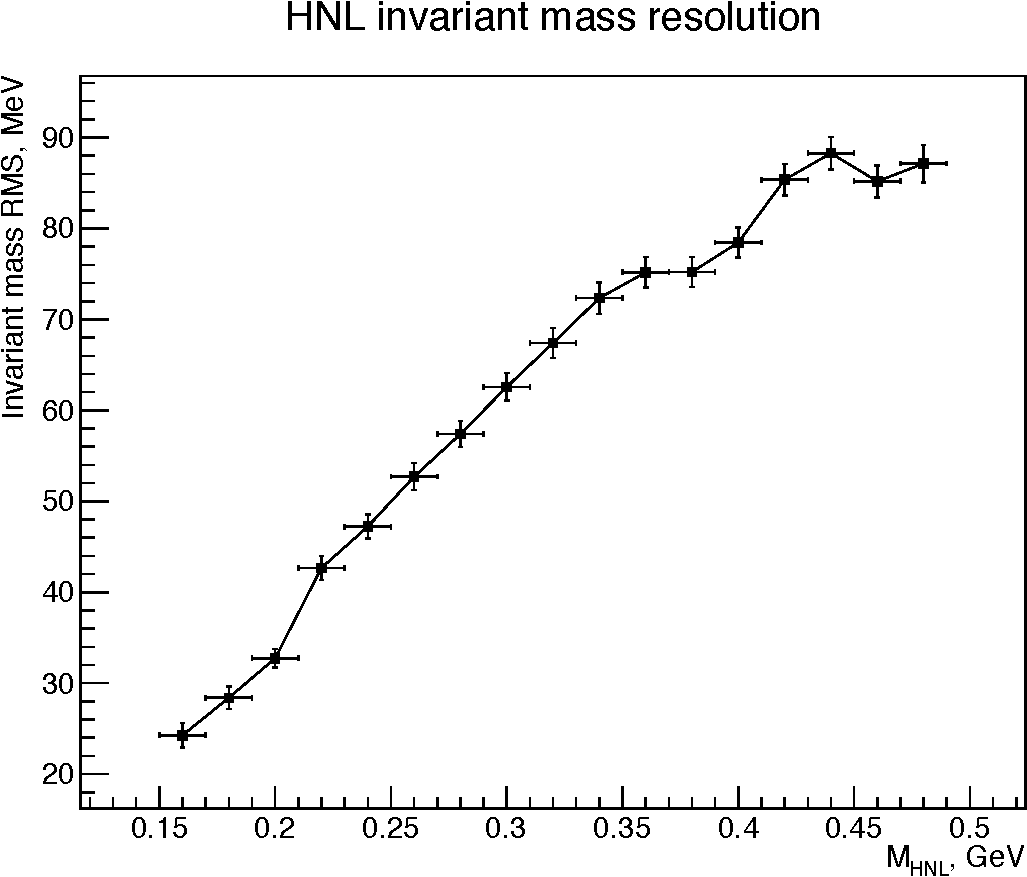
\includegraphics[width=\linewidth]{InvMassElePlot} \\ b) }
    \end{minipage}
    \caption{HNL invariant mass resolution (RMS) dependence on the HNL mass for (a) $N\to \mu\pi$ mode and (b) $N\to e\pi$ mode.}
    \label{fig:HNL:InvMassPlot}
\end{figure}

The second method requires significant background suppression. Usage of the gaseous TPC will provide very few neutrino interactions in the fiducial volume comparing to the scintillator detectors. Also the reconstruction of the heavy neutrino momentum direction could help a lot with the active neutrino events rejecting. We expect the HNL to be extremely collinear to the beam, while $\mu\pi$ pairs from the neutrino interactions will be distributed in the much wider angle. The details of the cut sequence are presented in the~\autoref{sec:HNL:sel}.

Thus we could perform a search of a few signal events in an extremely low background environment ($\approx1$). The details of the used statistical approach could be found in~\autoref{sec:HNL:stat}.


\chapter{HNL flux simulations}

First of all we need to estimate the sensitivity to mixing elements in our experiment. So we need to evaluate the HNL flux at the ND280. We decided to use the results of the neutrino flux simulation that was developed for the oscillation analysis within the T2K experiment. With this simulation we have all the information about the neutrinos entering the ND280 and their parent particles. Because of the kinematics the phase space of the meson decay into HNL is more limited then the decay into massless neutrino. E.g. the maximum angle of the HNL direction with respect to the parent meson direction is lower comparing to the massless neutrino case. Thus if we consider only mesons that could produce neutrino entering ND280 and omit all the others, we will definitely take all the possible HNL parent particles.

For the heavy neutrino simulation we take the particular meson decay and reweight is taking into account new kinematic and the branching ratios. Thus we will obtain the heavy neutrino spectrum in our detector.

\section{T2K flux simulation}
The accurate prediction of the neutrino flux is extremely important for the precise oscillation analysis. That's why the T2K collaboration have spent great effort on tuning the flux simulation in the most accurate way~\cite{Abe2013}. All the elements of the neutrino beamline (\autoref{ch:T2K:nu_beam}) are taken into account. The most tricky part is the evaluation of the meson production through the proton interactions in the carbon target. To reduce the systematic uncertainties the measurements from the NA61/SHINE experiment are used~\cite{Collaboration2018}.

\todo{details about NA61}.

The flow diagram of the neutrino flux simulation is shown in~\autoref{fig:HNL:nu_flux_sim}.

\begin{figure}[!ht]
    \centering
    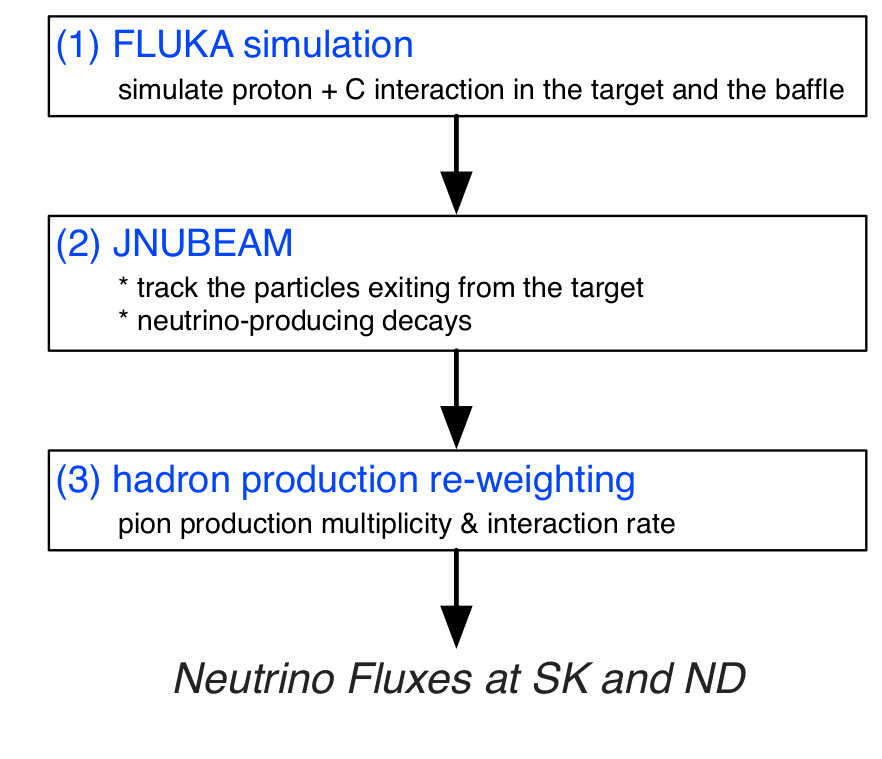
\includegraphics[width=0.5\linewidth]{nu_flux_sim}
    \caption{The neutrino flux prediction flow}
    \label{fig:HNL:nu_flux_sim}
\end{figure}

The proton beam spatial distribution and divergence are measured in the beamline monitors. The FLUKA generator is used to perform the simulation of the hadron interaction with the target and a buffle. Incident protons are set at known position and with kinetic energy of 30 GeV. The information of the generated particles that exited the simulated volume it stored. The next step is a JNUBEAM generator that takes the information about the particles from the previous step and tracks them through the horns and helium vessel, decay volume and surrounding concrete until the decay or the kinetic energy drop down below the threshold (10 MeV). At this step $\pi^\pm$, $K^\pm$, $K_L^0$ and $\mu^\pm$ decays are considered as neutrino sources. In order to save the computing time, the daughter neutrino is pointing towards the detector plane and the appropriate kinematic weight is assigned to the event.


After such simulation chain is performed and the outgoing neutrino is saved the hadronic chain in each event is reweighted based on the hadron interaction measurements. In our studies we are particularly interested in the kaon production. The generated kaon phase space and the coverage of the NA61 measurements are presented in~\autoref{fig:HNL:kaon_ps}.

After the reweighing of the hadron chains the total accuracy of the prediction is evaluated. The main systematic errors come from the hadronic interactions, primary beam alignment, horn current and magnetic field. The resulting uncertainty of the neutrino flux predictions are shown in~\autoref{fig:HNL:nu_flux_uncert}.

\begin{figure}[!ht]
    \begin{minipage}[!ht]{0.49\linewidth}
        \centering
        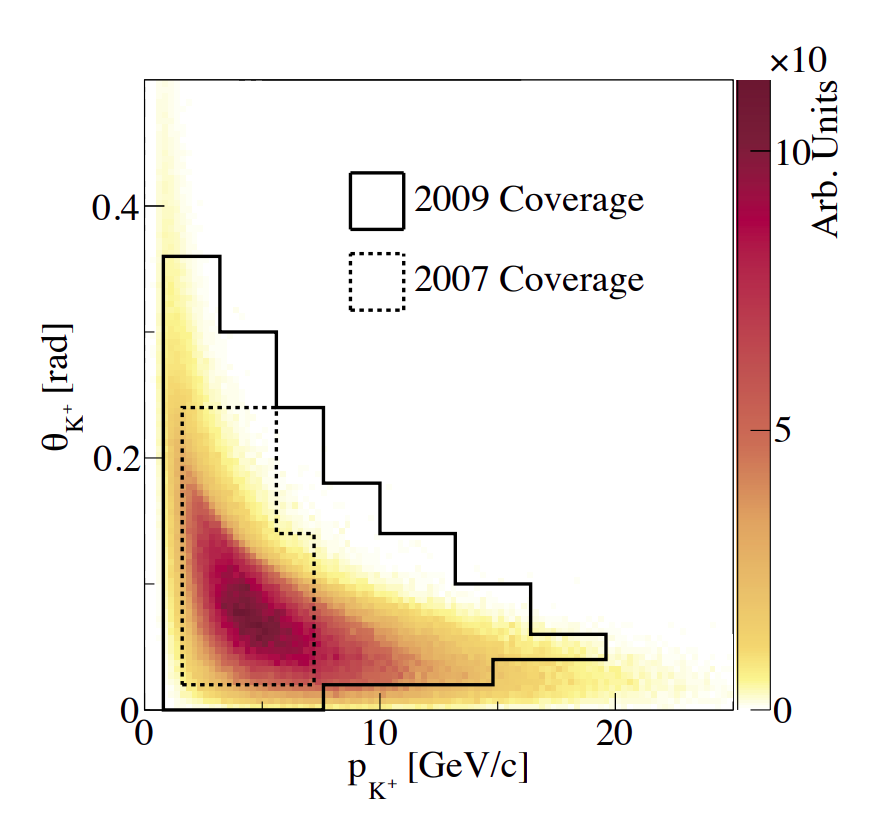
\includegraphics[width=\linewidth]{nu_flux_kaons}
        \caption{The phase space of positive kaons contributing to the predicted neutrino flux and the regions covered by the NA61/SHINE.}
        \label{fig:HNL:kaon_ps}
    \end{minipage}
    \hfill
    \begin{minipage}[!ht]{0.49\linewidth}
        \centering
        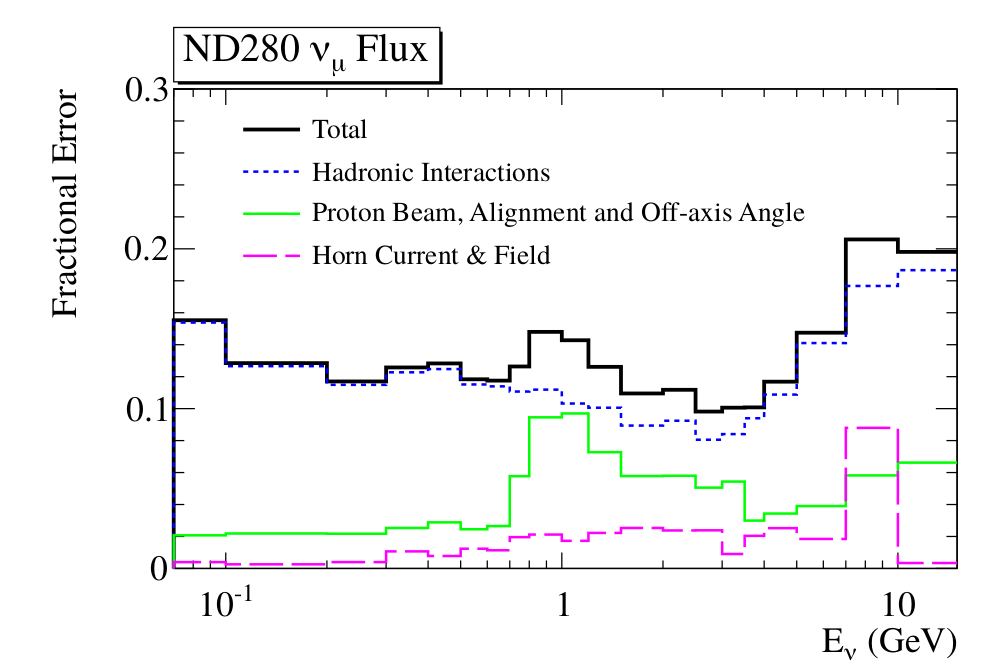
\includegraphics[width=\linewidth]{nu_flux_uncert}
        \caption{Fractional errors for the neutrino (left) and anti-neutrino (right).}
        \label{fig:HNL:nu_flux_uncert}
    \end{minipage}
\end{figure}


\section{HNL production}

For the propose of our study we would like to reweight the kaons decays based on the new kinematics and branching ratios. But we want to keep all the fine-tuning described in the previous section in order to keep the uncertainties as small as possible. Looking at the~\autoref{fig:HNL:nu_flux_sim}, we would like to change ``(2) JNUBEAM: neutrino-producing decays'', but to keep everything else at place.

Every neutrino event in original files has a weight, which was calculated as
\begin{equation}
    weight_{K\mu2}=scale_{POT}\cdot weight_{geom}\cdot P_{save}^{-1}\cdot Br_{K\mu2},
\end{equation}
where
\begin{itemize}
    \item $scale_{POT}$ --- $10^{21}$ POT normalization;
    \item $weight_{geom}$ --- probability of neutrino getting to the certain point of the detector plane, which was selected randomly;
    \item$P_{save}^{-1}$ --- probability to save event, in order to have results of MC model in a wide spectrum;
    \item $Br_{K\mu2}$ --- branching of $K\rightarrow\mu\nu_{\mu}$ decay.
\end{itemize}

For the HNL we need to save $scale_{POT}$ and $P_{save}^{-1}$ but recalculate $weight_{geom}$ and decay branching, so the weight of HNL event is
\begin{equation}
    weight_{K\rightarrow \ell+N}=weight_{K\mu2}\cdot\frac{weight_{geom,new}}{weight_{geom,old}}\cdot \frac{Br_{K\rightarrow \ell+N}}{Br_{K\mu2}},
    \label{eq:HNL:weightDif}
\end{equation}
where $weight_{geom,old}$ is calculated applying $M_{HNL}=0$ and $Br_{K\rightarrow \ell+N}$ is computed according to~\cite{Gorbunov2007}. The mixing element is just a multiplier and we assume it is equal to 1.

The new branching ratio is calculated according to~\cite{Gorbunov2007}:
\begin{equation}
    \begin{split}
    Br(K\rightarrow \ell+N)&=\frac{G_F^2 V_{us}^2 f_K^2 M_K M_{HNL}^2}{8\pi\hbar}\left(1-\frac{M_{HNL}^2}{M_K^2}+\frac{2M_\ell ^2}{M_K^2}+\frac{M_\ell^2}{M_{HNL}^2}\left(1-\frac{M_\ell^2}{M_K^2}\right)\right) \\
&\sqrt{\left(1+\frac{M_{HNL}^2}{M_K^2}-\frac{M_\ell^2}{M_K^2}\right)^2-\frac{4M_{HNL}^2}{M_K^2}} \cdot\tau_K,
    \end{split}
    \label{eq:HNL:Kdecay}
\end{equation}
where $G_F$ is Fermi constant, $V_{us}$ is a CKM matrix element, $M_\ell$ and $M_{HNL}$ are the lepton and the HNL masses, $M_K, f_K, \tau_K$ are kaon mass, form-factor, lifetime respectively.

HNL enters the detector front plane randomly. The geometry weight is calculated as a probability of a daughter particle to have a momentum with a certain angle $\theta$ w.r.t. the parent momentum. Modifying
\begin{eqnarray}
    weight_{geom,new}=weight_{geom, lab}=\frac{p_{lab}E_{cm}}{p_{cm}^2}\cdot weight_{geom,cm}
    \nonumber \\
    weight_{geom, cm} = \frac{1}{4\pi}\delta\left(p-p_{cm}\right)
\end{eqnarray}
we finally got
\begin{equation}
    weight_{geom, lab}=\frac{1}{4\pi}\frac{p_{lab}E_{cm}}{p_{cm}^2}\frac{cos\theta_{lab}\left(\beta/\beta_{lab}\pm\sqrt{1+\gamma^2\left(1-\left(\beta/\beta_{lab}\right)^2\right)tg^2\theta_{lab}}\right)}{\gamma\left(1-\beta^{2}cos^{2}\theta_{lab}\right)}.
    \label{eq:HNL:lorentz}
\end{equation}

Here we assume that the HNL's lifetime is rather large enough to reach the ND280. There are two reasons for such assumption:
\begin{itemize}
    \item if the HNL mean free path is shorter, it will dramatically reduce the HNL flux at ND280 and the sensitivity will be rather poor;
    \item short lifetime doesn't allow to calculate probability of the HNL decay in TPC like~\autoref{eq:HNL:Pdecay} and make study more complicated, because life time $\tau$ depends on mixing element
\end{itemize}
From the cosmology~\cite{Gorbunov2007} we have an upper bound on the HNL lifetime  $\tau < 0.1s$, which is mainly based on the baryogenesis models. So for the current analysis we have the HNL lifetime region $1\mu s\ll\tau<0.1s$ which is wide enough. An estimation of the corresponding mean free path of the HNL gives $\Lambda_{HNL}=c\beta\gamma\tau\gg280 m$.

To cross-check our kinematic model we compare the HNL spectra for $M_{HNL}=0$ with the active neutrino spectrum from $K\mu2$ and make sure that they are identical. After performing modeling of all kaon decays we get the HNL spectra at the ND280 entrance plane (\autoref{fig:HNL:fluxKpos}).
\begin{figure}[!ht]
    \begin{minipage}{0.49\linewidth}
        \center{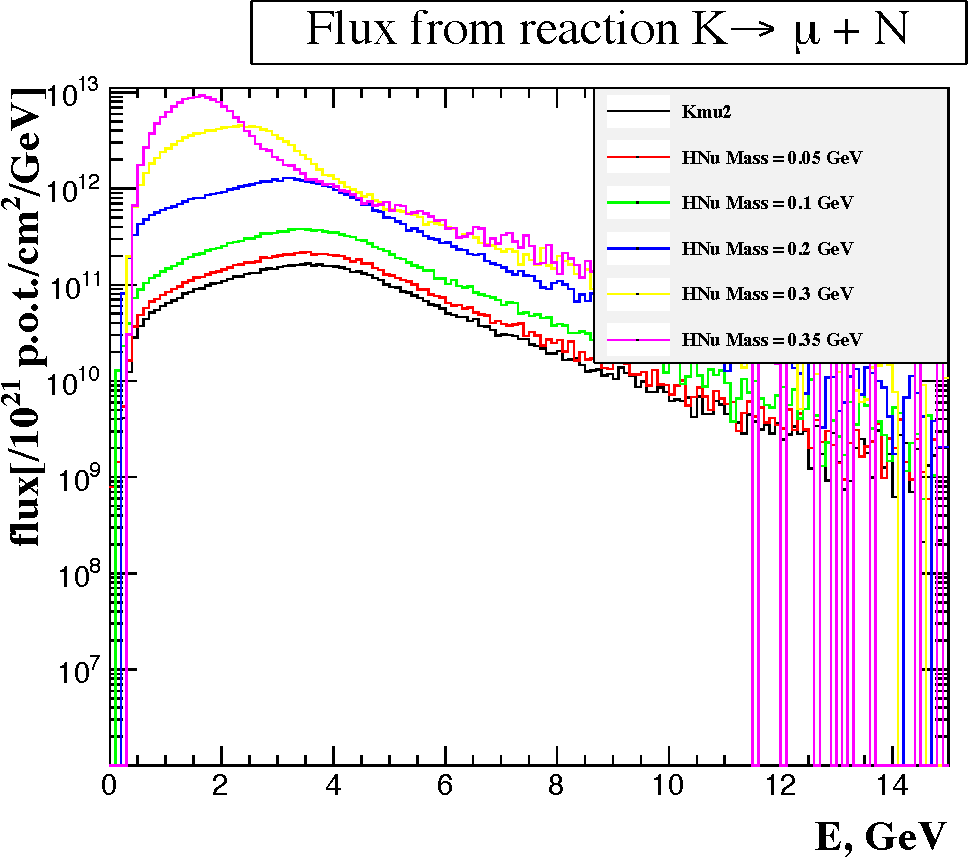
\includegraphics[width=\linewidth]{fluxKmu} \\ $K^+\rightarrow \mu^+N$}
    \end{minipage}
    \hfill
    \begin{minipage}{0.49\linewidth}
        \center{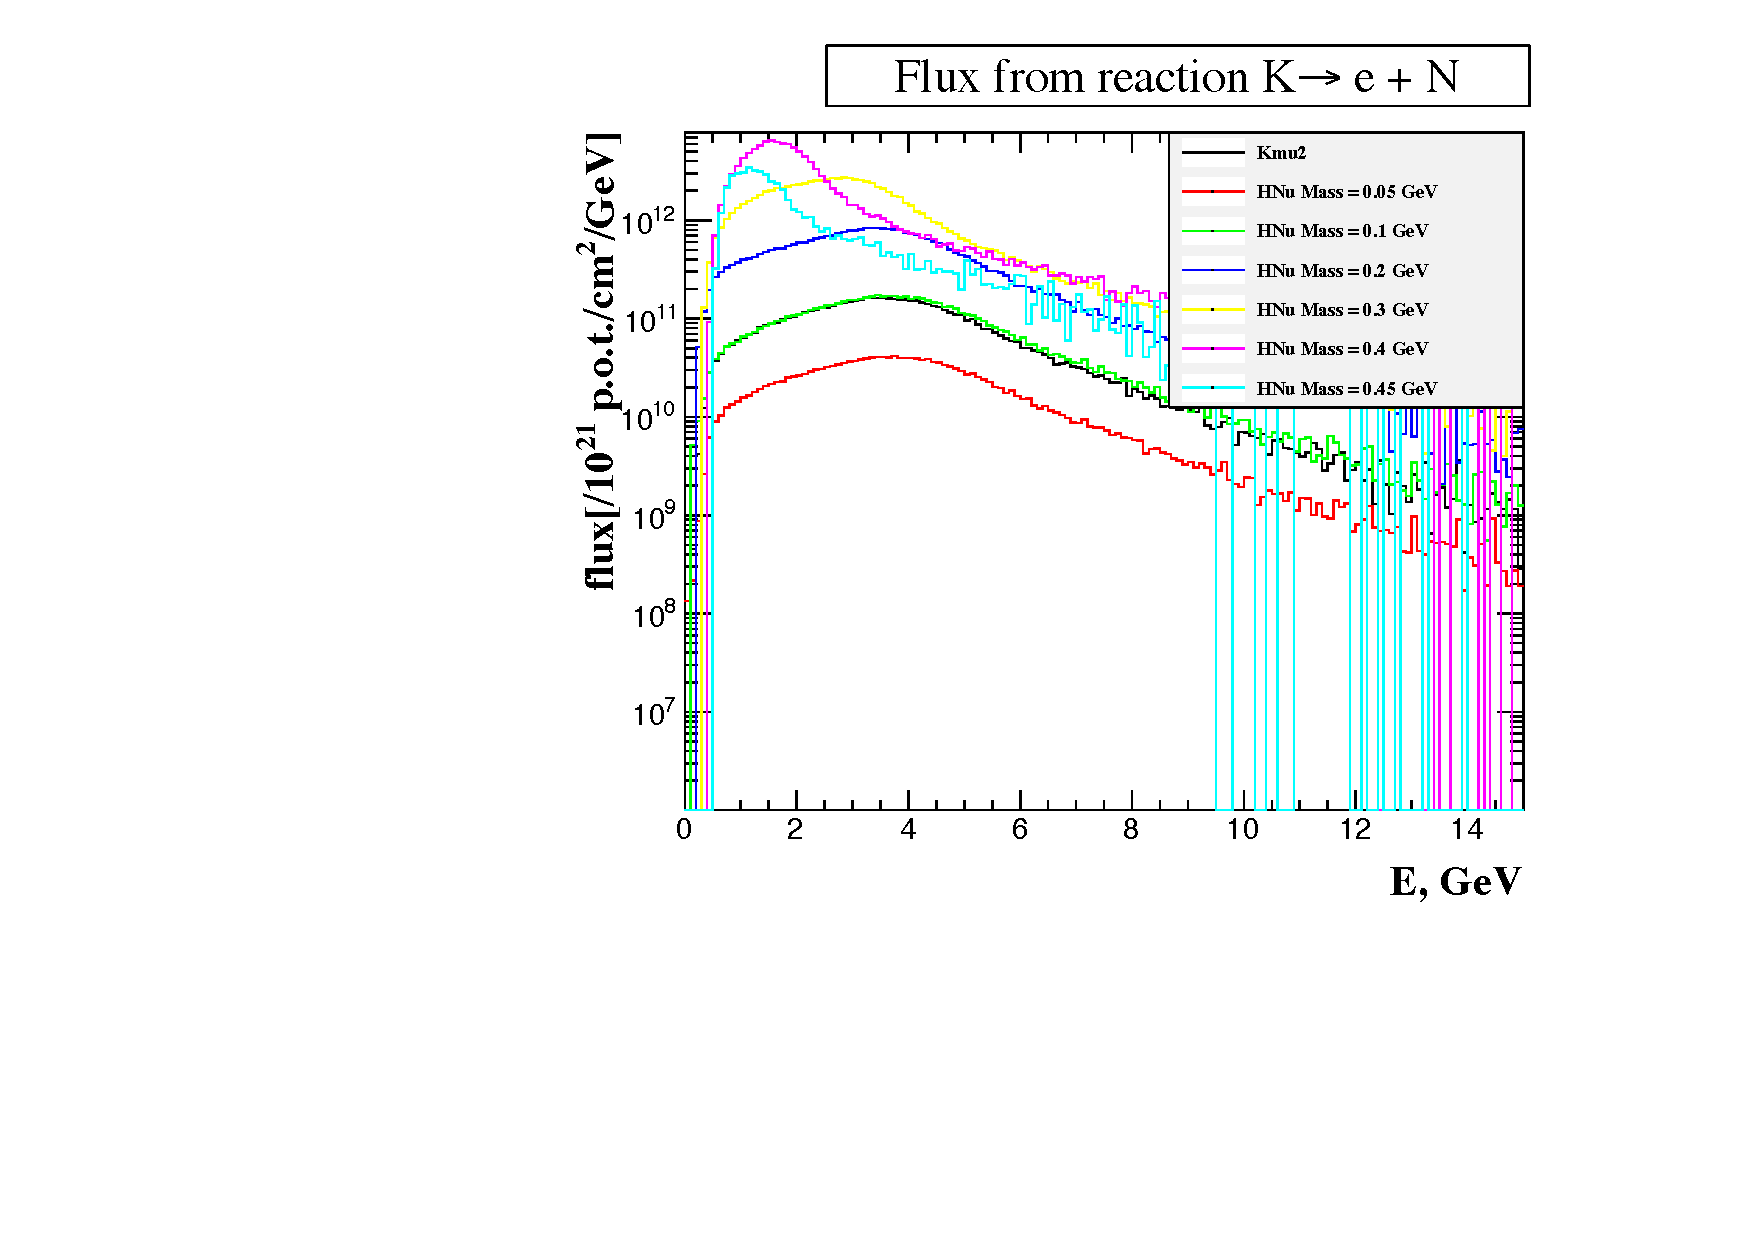
\includegraphics[width=\linewidth]{fluxKe} \\ $K^+\rightarrow e^+N$}
    \end{minipage}
    \caption{HNL energy spectra at the ND280 front plane for two modes: $K^+\rightarrow \mu^+N$ and $K^+\rightarrow e^+N$ for the different HNL masses.}
    \label{fig:HNL:fluxKpos}
\end{figure}

There are two effects, that cause the flux difference comparing to the active neutrino flux (\autoref{eq:HNL:weightDif}). The first one is ``massive'' kinematic of the parent meson decay. This correction is calculated according to~\autoref{eq:HNL:lorentz}. This impact is shown in~\autoref{fig:HNL:fluxMassKpos}. The branching ratio is assumed equal to 1.
\begin{figure}[!ht]
    \begin{minipage}{0.49\linewidth}
        \center{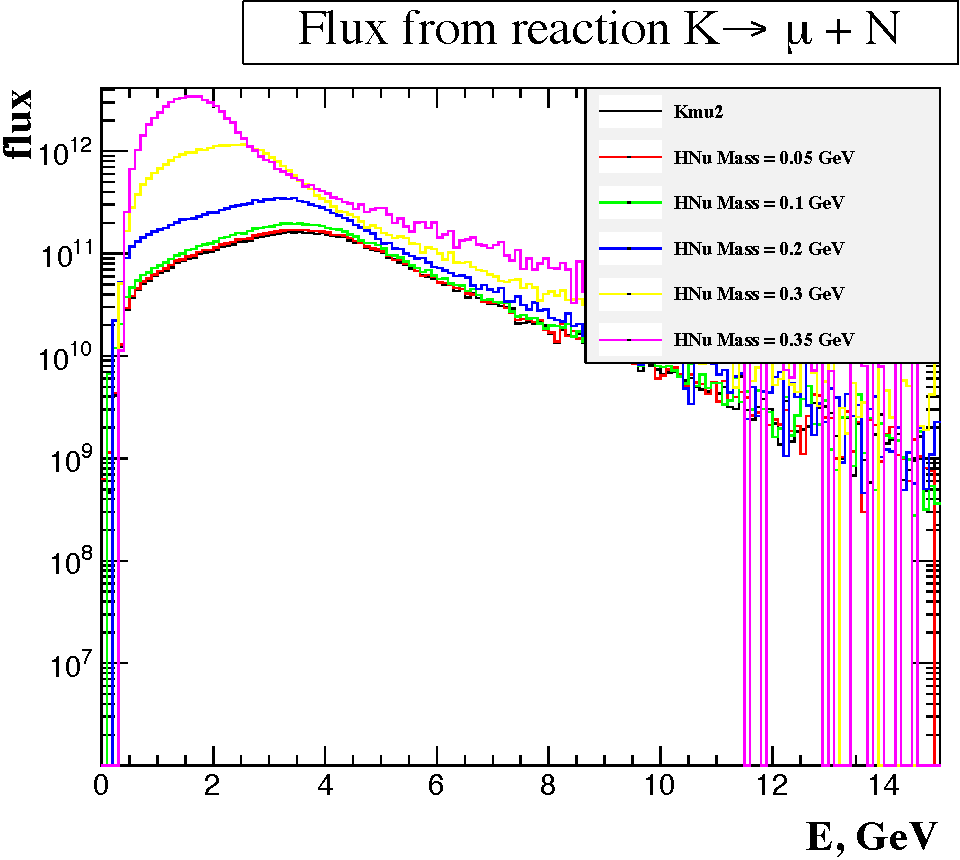
\includegraphics[width=\linewidth]{fluxMassKmu} \\ $K^+\rightarrow \mu^+N$}
    \end{minipage}
    \hfill
    \begin{minipage}{0.49\linewidth}
        \center{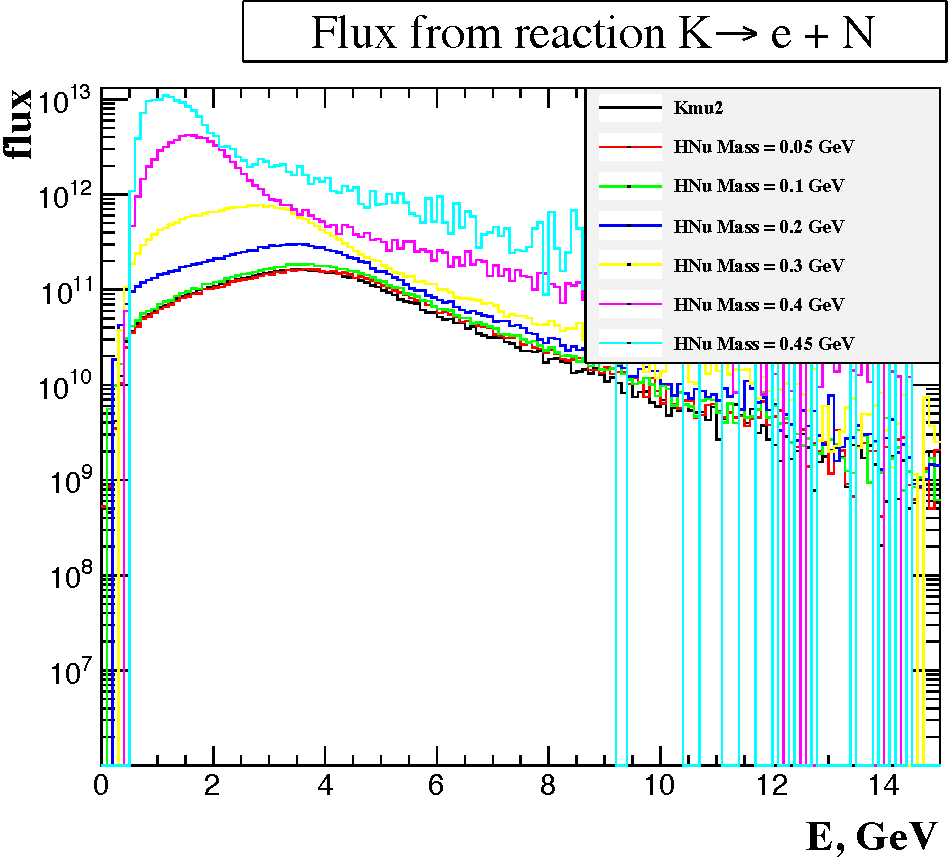
\includegraphics[width=\linewidth]{fluxMassKe} \\ $K^+\rightarrow e^+N$}
    \end{minipage}
    \caption{HNL spectra at the ND280 front plane for two modes and for the different HNL masses assuming the branching ratios equal to 1.}
    \label{fig:HNL:fluxMassKpos}
\end{figure}

The second effect is the modification of the branching ratio of the kaon decay. It is calculated according to~\autoref{eq:HNL:Kdecay}. The branching ratio dependence is shown in Fig.~\ref{fig:HNL:KdecayBR}.
\begin{figure}[!ht]
    \begin{minipage}[!ht]{0.49\linewidth}
        \center{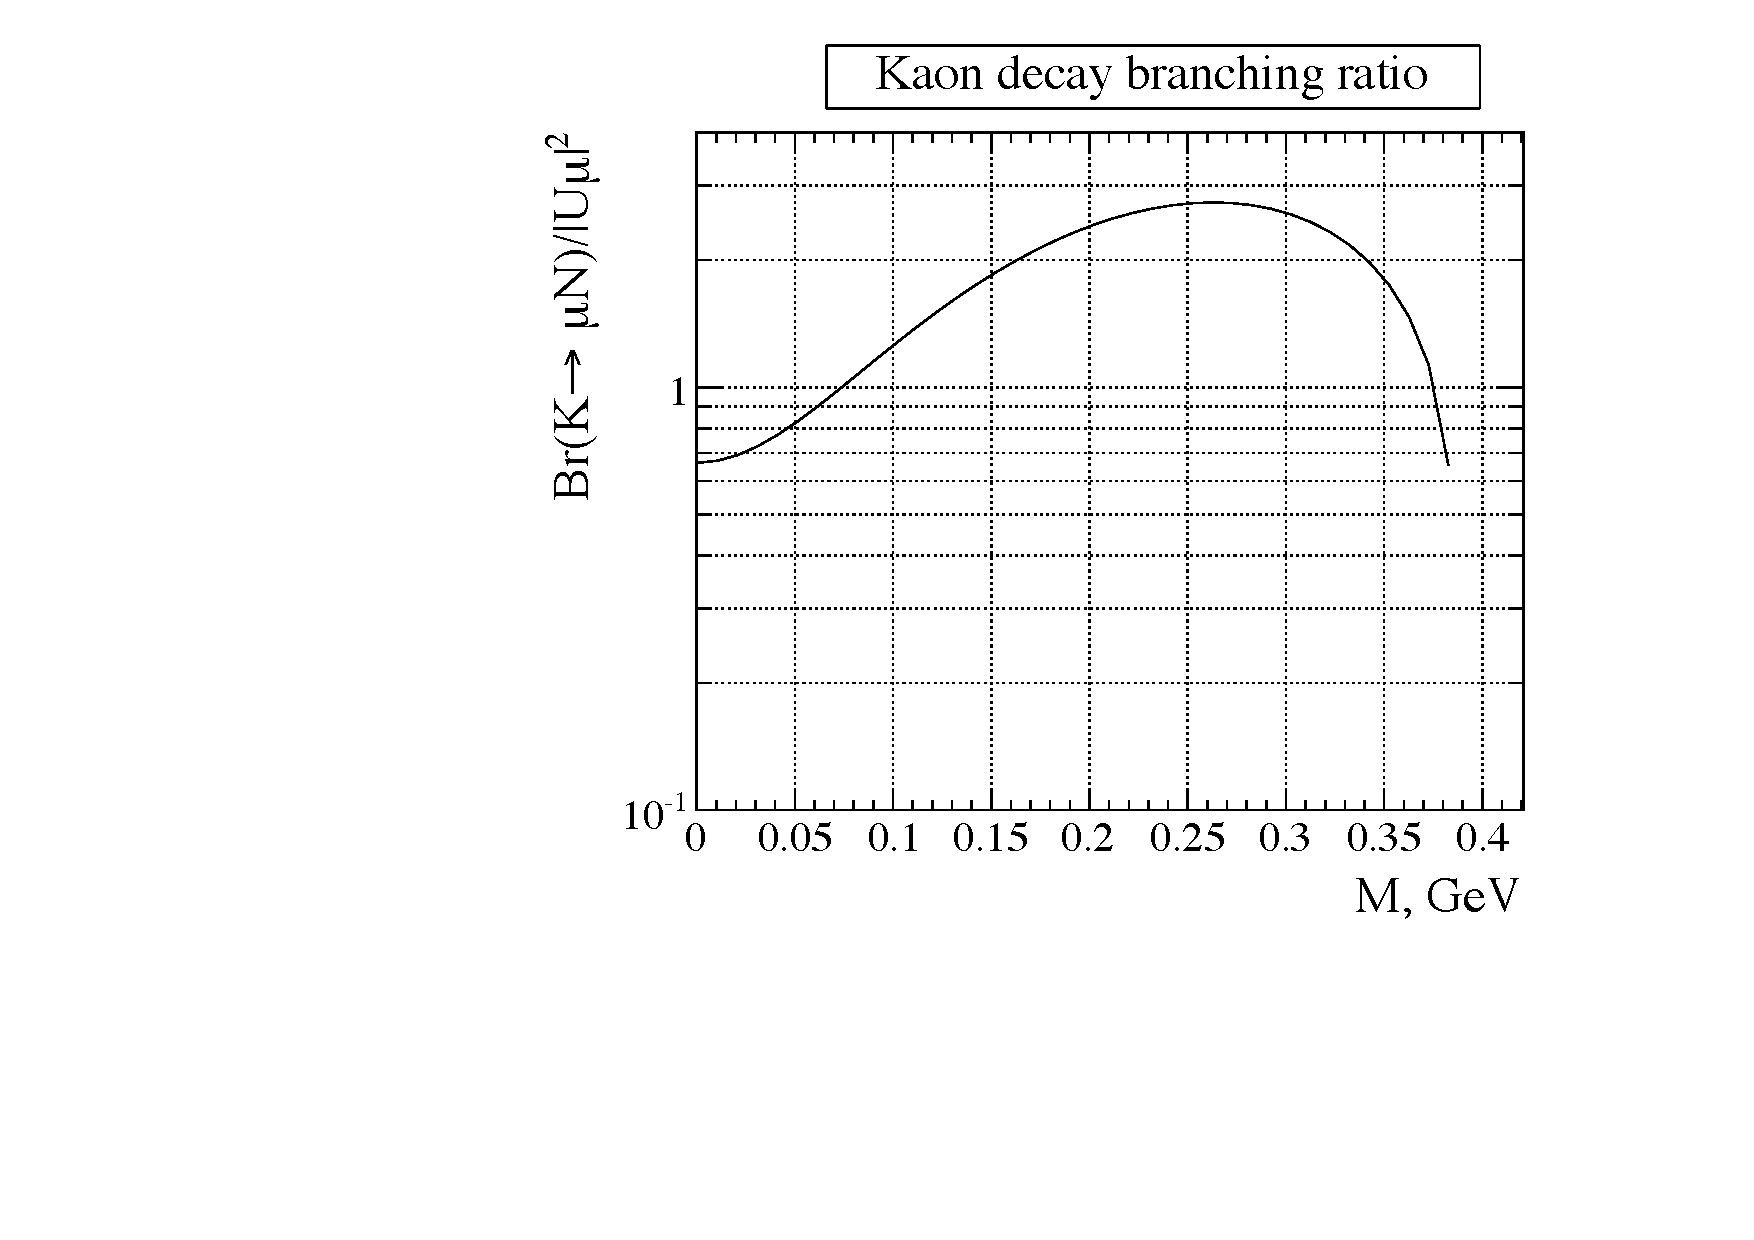
\includegraphics[width=\linewidth]{BrKMu} \\ a)}
    \end{minipage}
    \hfill
    \begin{minipage}[!ht]{0.49\linewidth}
        \center{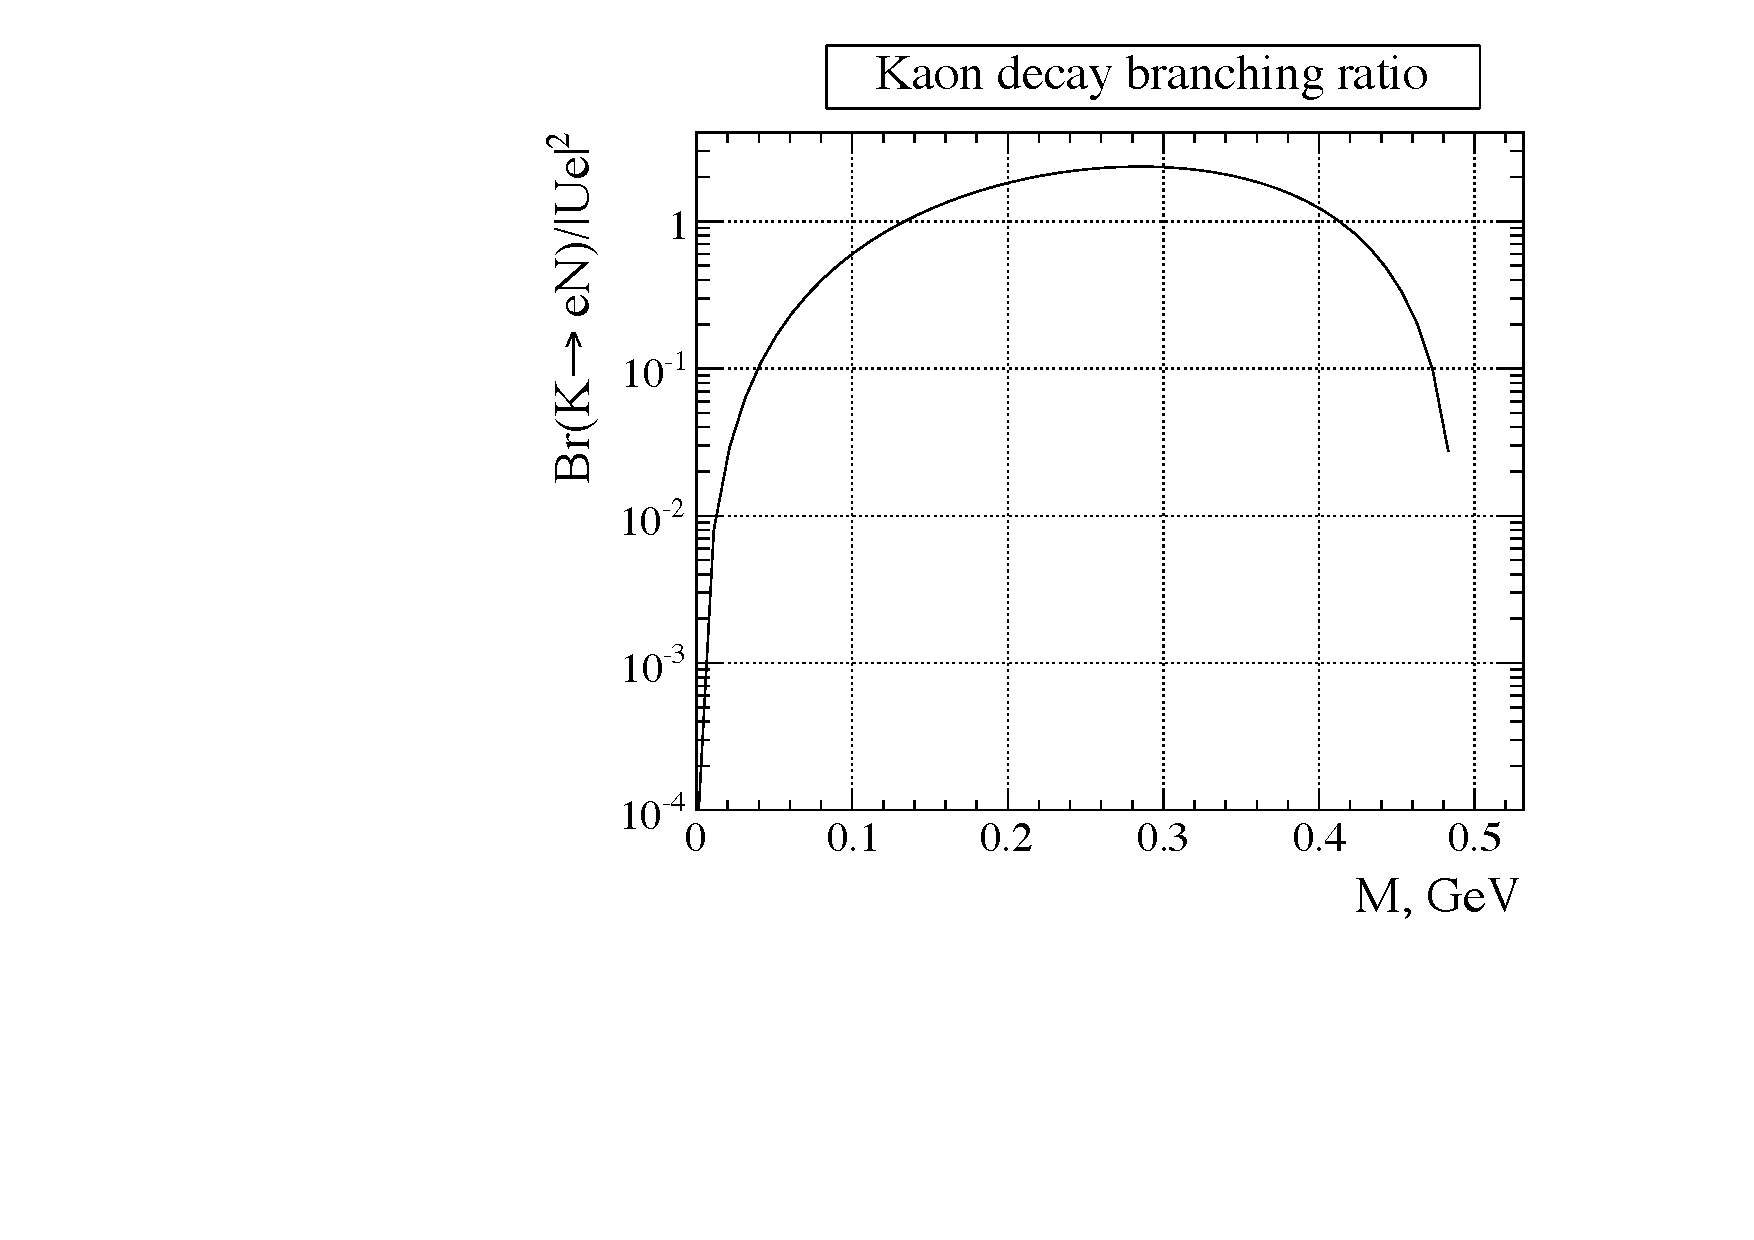
\includegraphics[width=\linewidth]{BrKEle} \\ b)}
    \end{minipage}
    \caption{Kaon decay branching ratio divided into the mixing element for two modes: (a) $K\to \mu N$ and (b) $K\to eN$.}
    \label{fig:HNL:KdecayBR}
\end{figure}

The difference of the time of flight for the active neutrino and HNL is described in the analysis~\autoref{sec:HNL:tof_corr}.

Since we study both $K^+$ and $K^-$ modes we compare HNL fluxes from both parent particles. The flux of HNL from $K^-$ decays is nearly three times lower than one from $K^+$ decays. It was expected since the cross section of $K^-$ production is approximately  tree times lower.

\section{HNL decays}

From the spectra of the heavy neutrinos, we can estimate the number of events from HNLs' decays and a sensitivity to mixing elements. As already described we just need the number of expected signal events. Number of decays is
\begin{equation}
    N_{events}=\phi(HNL/10^{21}p.o.t./cm^2)\cdot S_{det} \cdot P_{decay}^{TPC}\cdot Br_{mode},
    \label{eq:HNL:Nevents}
\end{equation}
where
\begin{itemize}
    \item $\phi(HNL/10^{21}p.o.t./cm^2)$ --- the HNL flux per $10^{21}POT$ per $cm^2$;
    \item $S_{det}$ --- area of the ND280 front plane;
    \item $P_{decay}^{TPC}$ --- the probability of a HNL decay in one of 3 TPCs;
    \item $Br_{mode}$ --- branching of a current decay mode.
\end{itemize}
The decay probability between two points with coordinates $z_1$ and $z_2$, assuming large mean free path, is
\begin{equation}
    P_{decay}(z_2-z_1)=exp(-\frac{z_1}{c\beta\gamma\tau})-exp(-\frac{z_2}{c\beta\gamma\tau})\approx \frac{z_2-z_1}{c\beta\gamma\tau}
    \label{eq:Pdecay}
\end{equation}
where $\tau$ is HNL lifetime. Taking into account that
\begin{equation}
    Br_{mode}=\frac{\Gamma_{mode}}{\Gamma_{total}}=\Gamma_{mode}\cdot\tau,
\end{equation}
finally have
\begin{equation}
    N_{events}=\phi(HNL/10^{21}p.o.t./cm^2)\cdot\frac{V_{FV}}{c\beta\gamma}\cdot\Gamma_{mode},
    \label{eq:HNL:EventsN}
\end{equation}
where $V_{FV}$ is a sum of the fiducial volumes of 3 TPC's. The decay width is calculated according to~\cite{Gorbunov2007, Johnson1997}. For 2-body decay we have
\begin{equation}
    \begin{split}
    \Gamma\left(N\to \pi^+\ell_\alpha^-\right)&=\frac{\left|U_\alpha\right|^2}{16\pi}G_F^2\left|V_{ud}\right|^2f_\pi^2M_HNL^3\left(\left(1-\frac{M_\ell^2}{M_HNL^2}\right)^2-\frac{M_{\pi}^2}{M_HNL^2}\left(1+\frac{M_\ell^2}{M_HNL^2}\right)\right)     \\
    &\times \sqrt{\left(1-\frac{\left(M_{\pi}-M_\ell\right)^2}{M_HNL^2}\right)\left(1-\frac{\left(M_{\pi}+M_\ell\right)^2}{M_HNL^2}\right)}
    \end{split}
\end{equation}
where  $\ell$ means lepton, $G_F$ --- Fermi constant, $f_\pi$ --- pion form-factor, $V$ --- CKM matrix element. The dependence of the decay width on the HNL mass is shown in~\autoref{fig:HNL:decBr}.

\begin{figure}[!ht]
    \begin{minipage}[!ht]{0.49\linewidth}
        \center{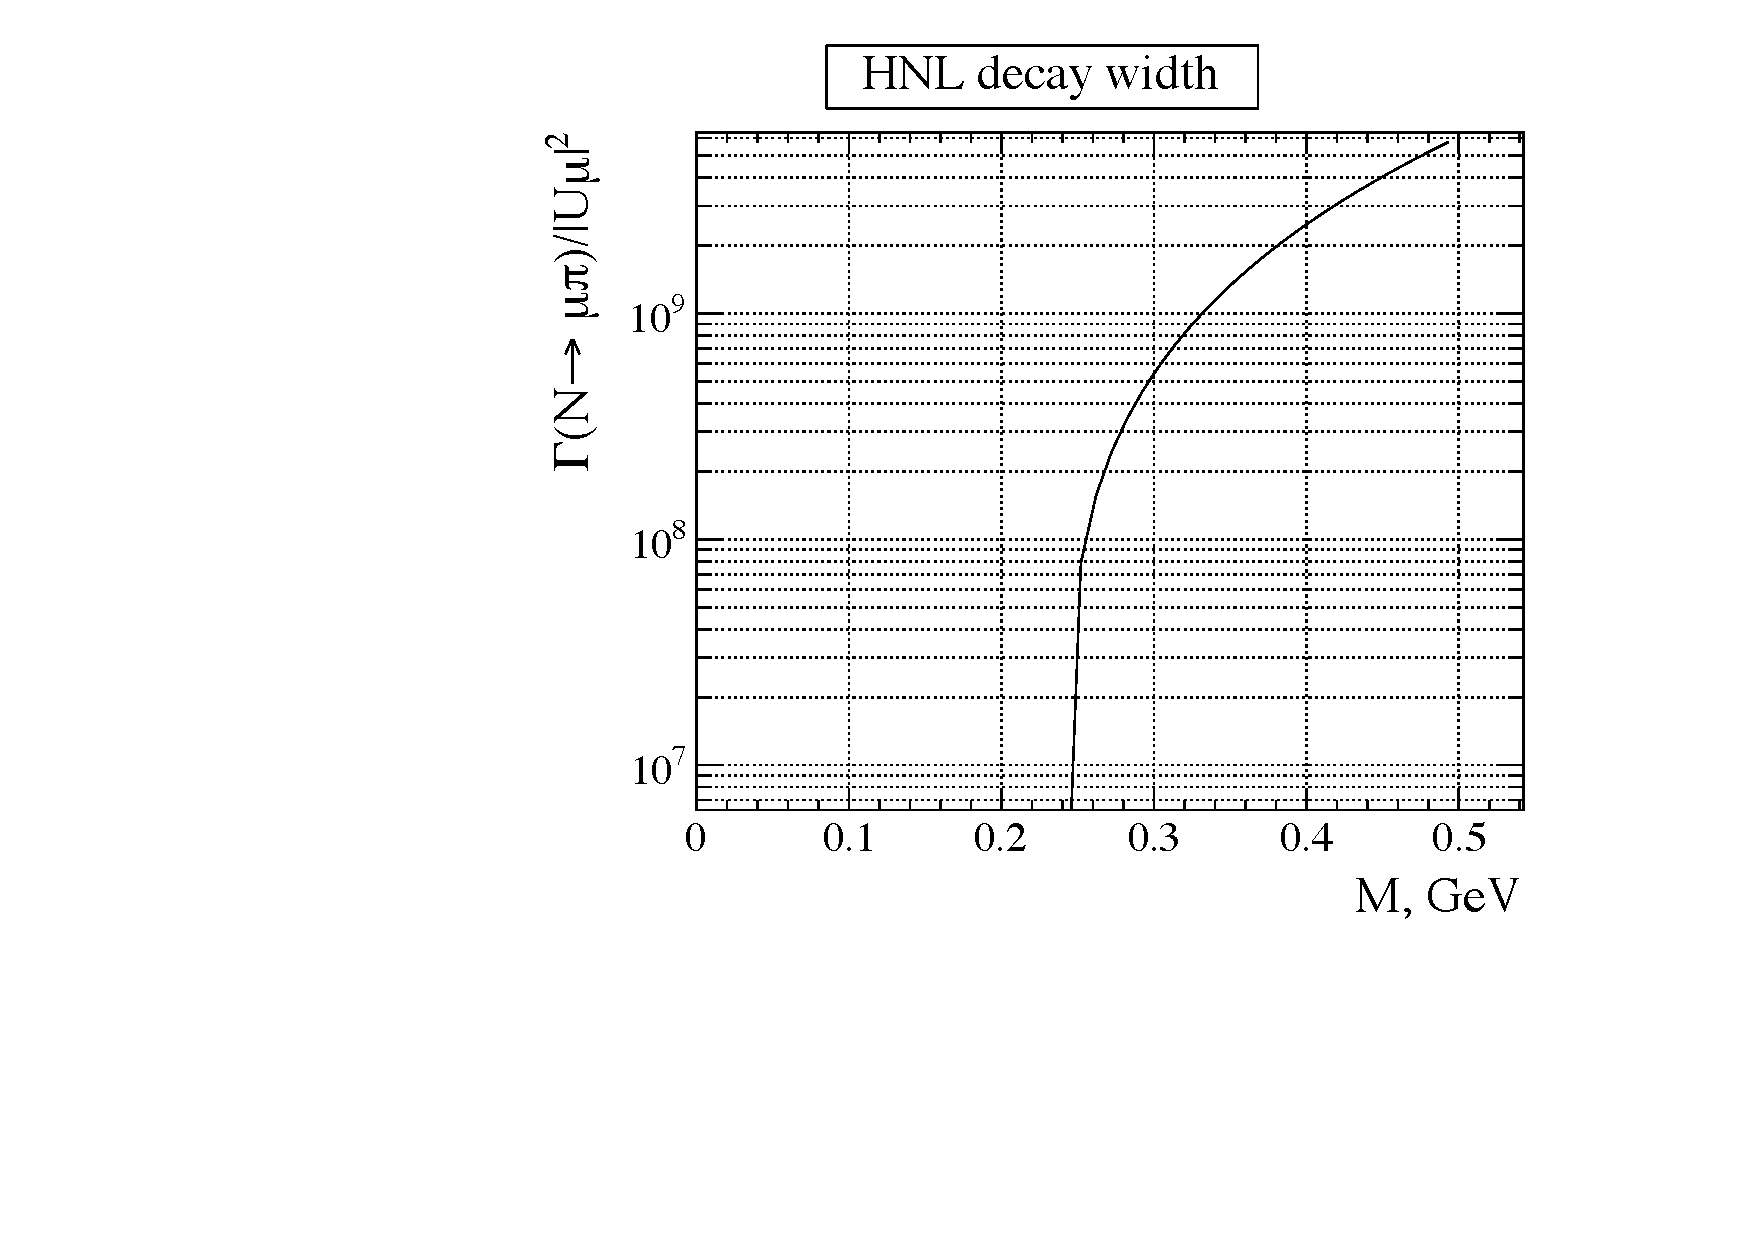
\includegraphics[width=\linewidth]{BrMu} \\ a)}
    \end{minipage}
    \hfill
    \begin{minipage}[!ht]{0.49\linewidth}
        \center{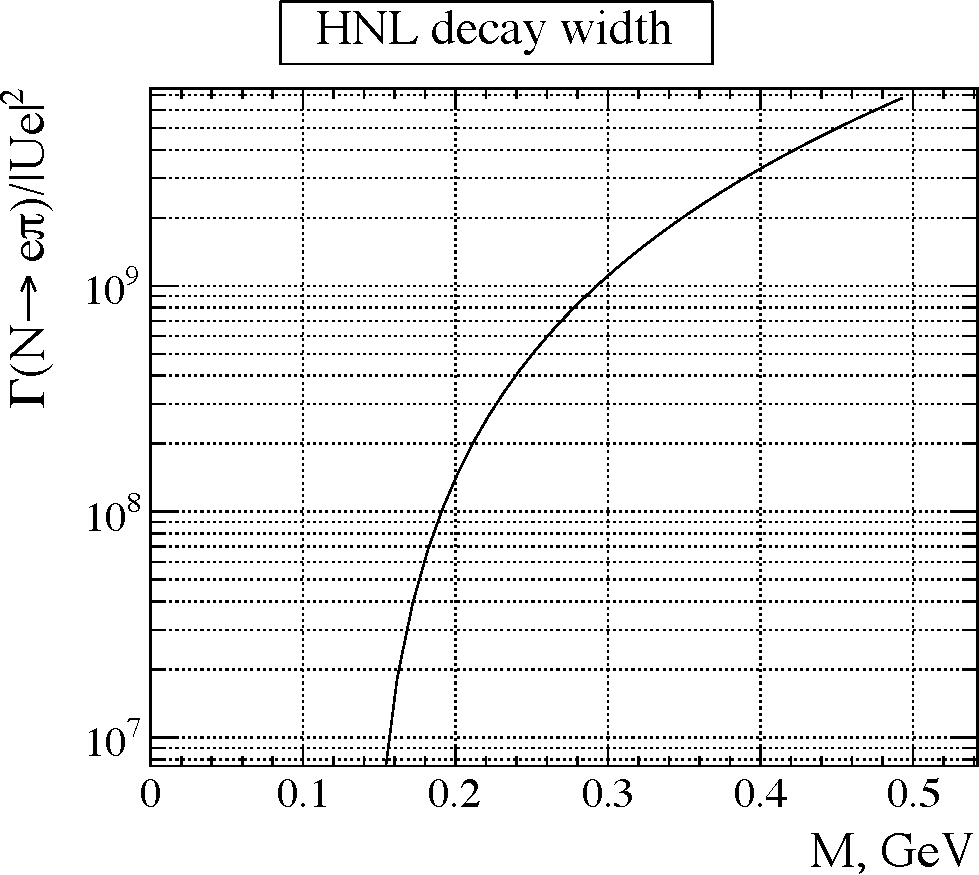
\includegraphics[width=\linewidth]{BrEle} \\ b)}
    \end{minipage}
    \caption{HNL decay width for two modes: (a) $N\to \mu\pi$ and (b) $N\to e\pi$ divided into the mixing element.}
    \label{fig:HNL:decBr}
\end{figure}

As $\phi\propto\left|U\right|^2$ and $\Gamma_{mode}\propto\left|U\right|^2$ our sensitivity (\autoref{eq:HNL:constraints}) for zero background and 100\% efficiency of HNL daughter detection is
\begin{equation}
    \left|U\right|^2_{limit}=\sqrt{\frac{2.3}{N_{events}}},
\end{equation}
Where 2.3 is a statistical coefficient for 90\% C.L. according to ~\cite{Cousins1992}. The sensitivity of our experiment for two body decays is shown in Fig.~\ref{fig:HNL:Ue2Umu2TwoBody}, ~\ref{fig:HNL:UeUmuTwoBody}, in green. It's compared with current limits from PS191~\cite{Bernardi1988} (in red) and Asaka et al prediction~\cite{Asaka2012} (in blue).
\begin{figure}[!ht]
    \begin{minipage}[!ht]{0.49\linewidth}
        \center{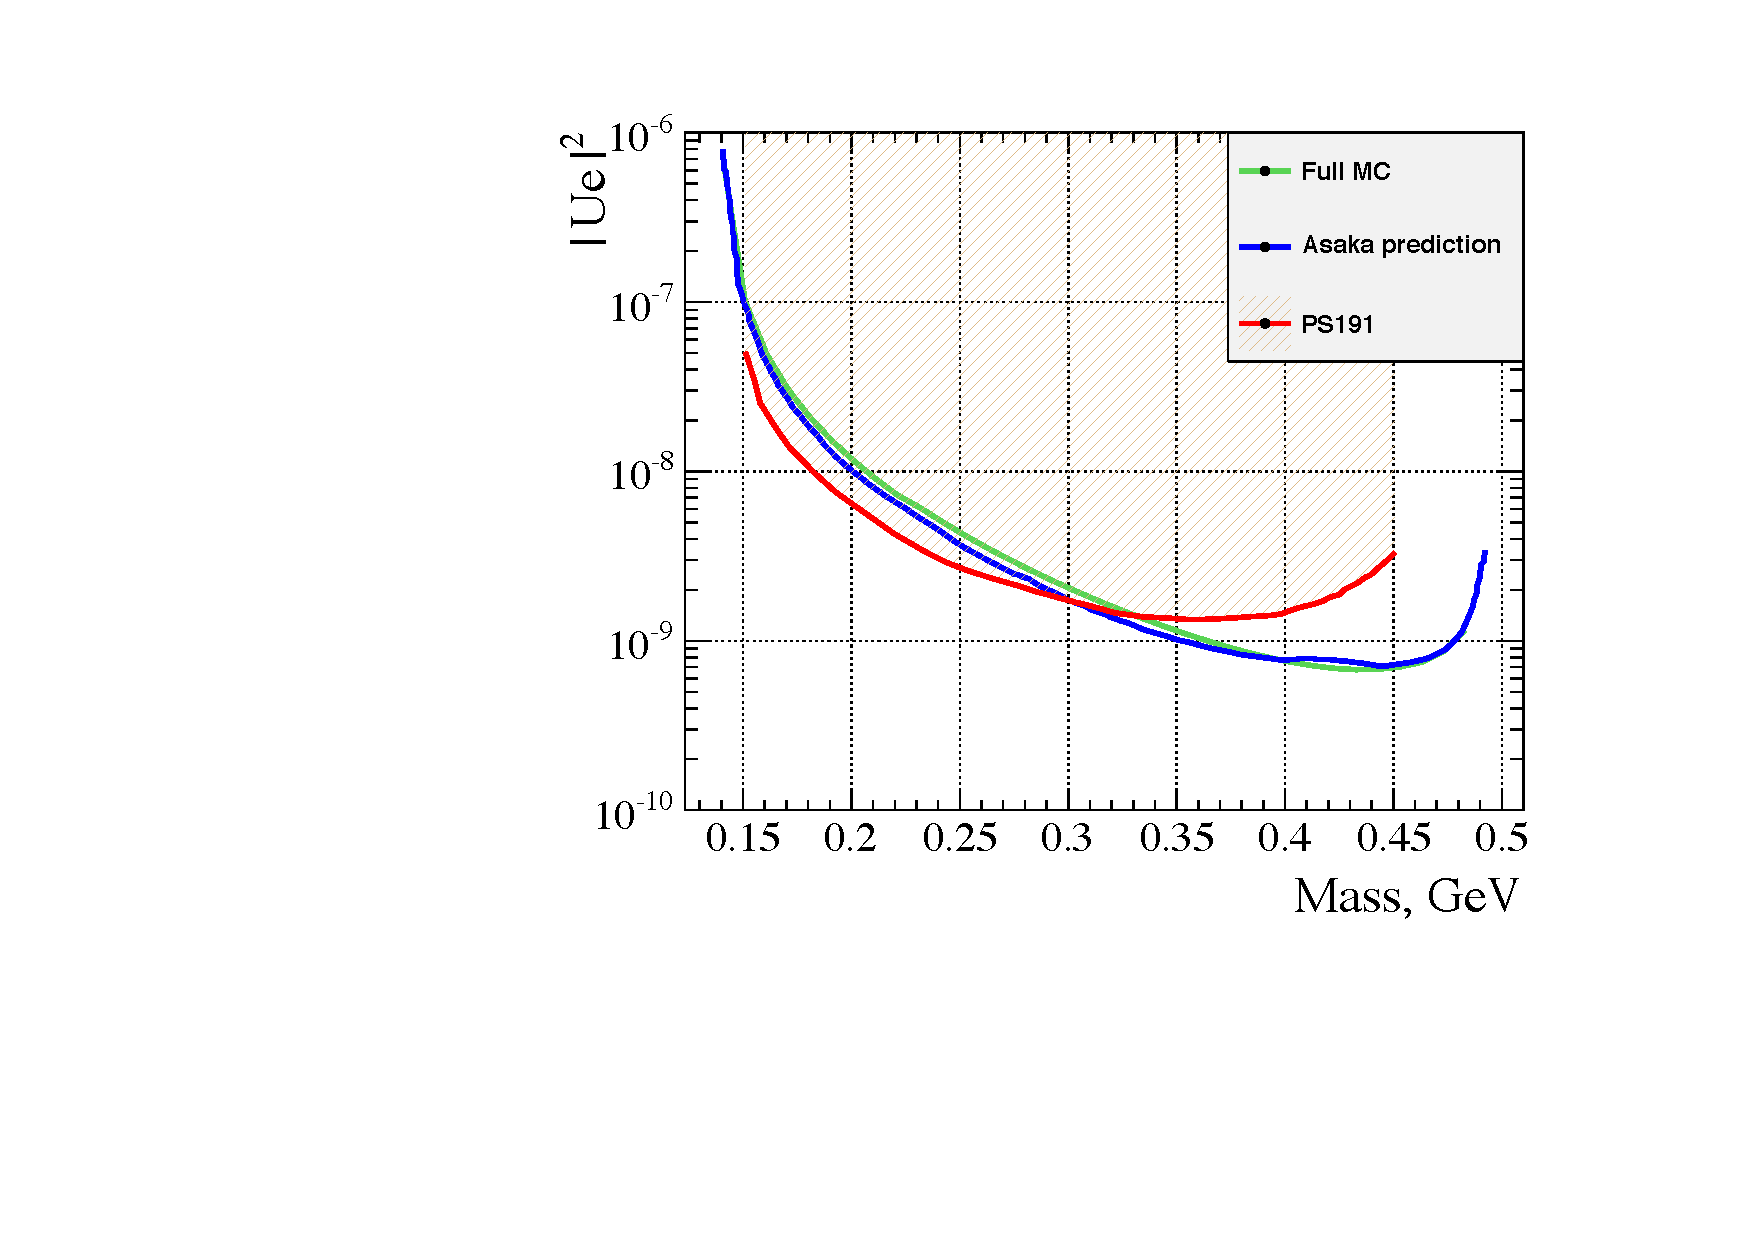
\includegraphics[width=\linewidth]{Ue2TwoBody} \\ a) $K\to eN\to e(e\pi)$}
    \end{minipage}
    \hfill
    \begin{minipage}[!ht]{0.49\linewidth}
        \center{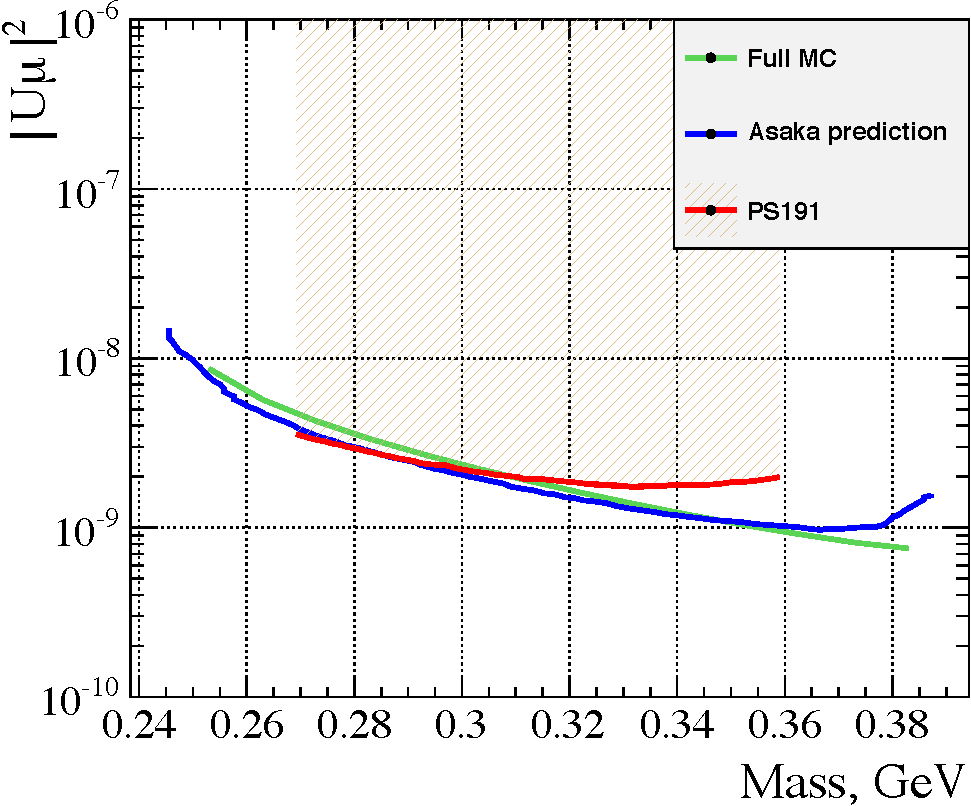
\includegraphics[width=\linewidth]{Umu2TwoBody} \\ b) $K\to\mu N\to \mu(\mu\pi)$}
    \end{minipage}
    \caption{Sensitivity of T2K to mixing element for two body decay modes for $10^{21}POT$. The detection efficiency of 100\% and no background are assumed.}
    \label{fig:HNL:Ue2Umu2TwoBody}
\end{figure}

\begin{figure}[!ht]
    \center{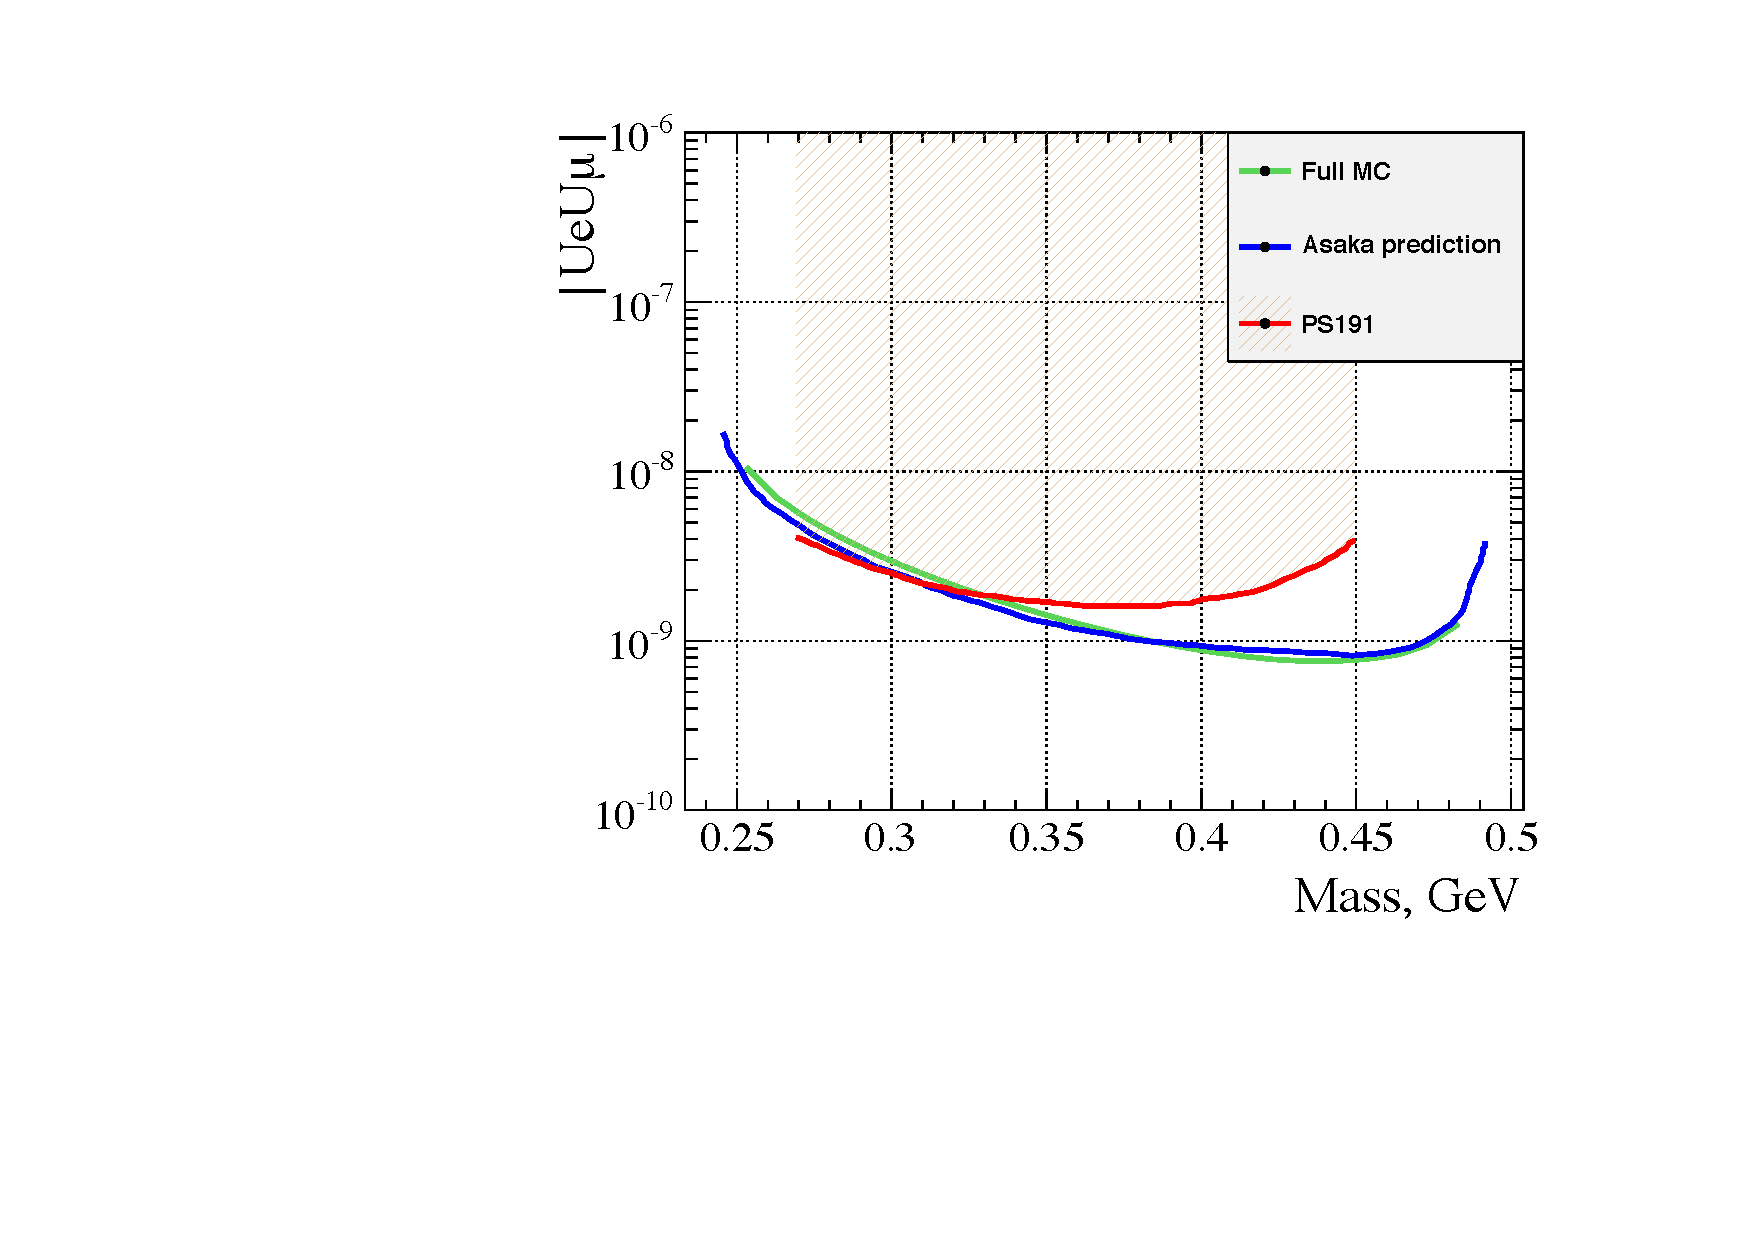
\includegraphics[width=0.49\linewidth]{UeUmuTwoBody}  \\ $K\to eN\to e(\mu\pi)$}
    \caption{Sensitivity of T2K to mixing element for two body decay modes for $10^{21}POT$. The detection efficiency of 100\% and no background are assumed.}
    \label{fig:HNL:UeUmuTwoBody}
\end{figure}

Three body decays of HNL were also studied. Possible improvement over the PS191 results is worse than for 2-body modes, the background for such events seems to be much larger due to the isotropic distribution of the charged daughter particles. In our study we will concentrate on 2-body decays and $N\to\mu\mu\nu$ mode. Three body sensitivity is shown in Fig.~\ref{fig:HNL:TreeBodyFirst} and Fig.~\ref{fig:HNL:ThreeBodySecond}.

\begin{figure}[!ht]
    \begin{minipage}[!ht]{0.49\linewidth}
        \center{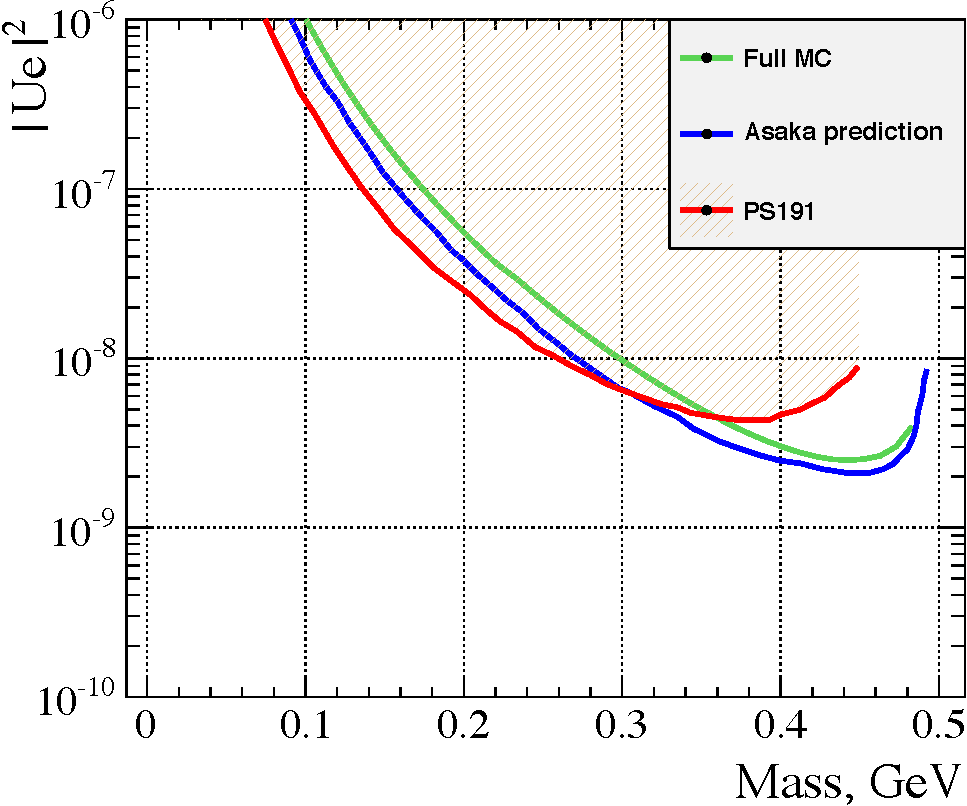
\includegraphics[width=\linewidth]{Ue2ThreeBody} \\ a) $K\to eN\to e(ee\nu_e)$}
    \end{minipage}
    \hfill
    \begin{minipage}[!ht]{0.49\linewidth}
        \center{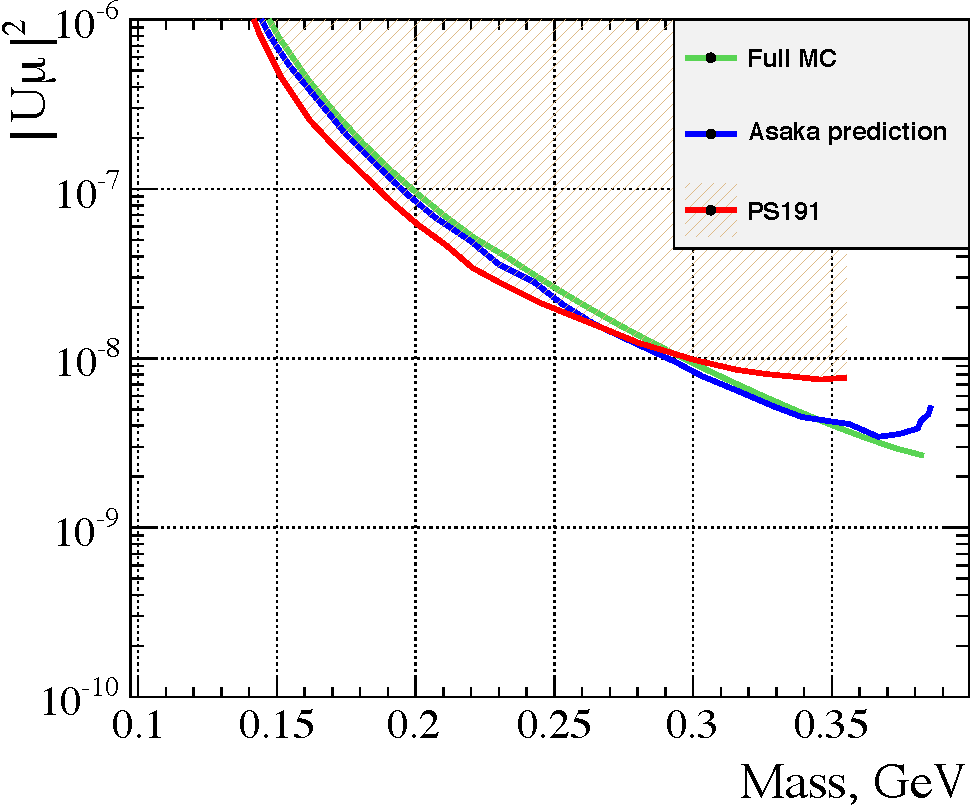
\includegraphics[width=\linewidth]{Umu2ThreeBody} \\ b) $K\to \mu N\to \mu(\mu e\nu_e)$}
    \end{minipage}
    \caption{Sensitivity of T2K to mixing element for three body decay modes for $10^{21}POT$. The detection efficiency of 100\% and no background are assumed.}
    \label{fig:HNL:TreeBodyFirst}
\end{figure}

\begin{figure}[!ht]
    \begin{minipage}[!ht]{0.49\linewidth}
        \center{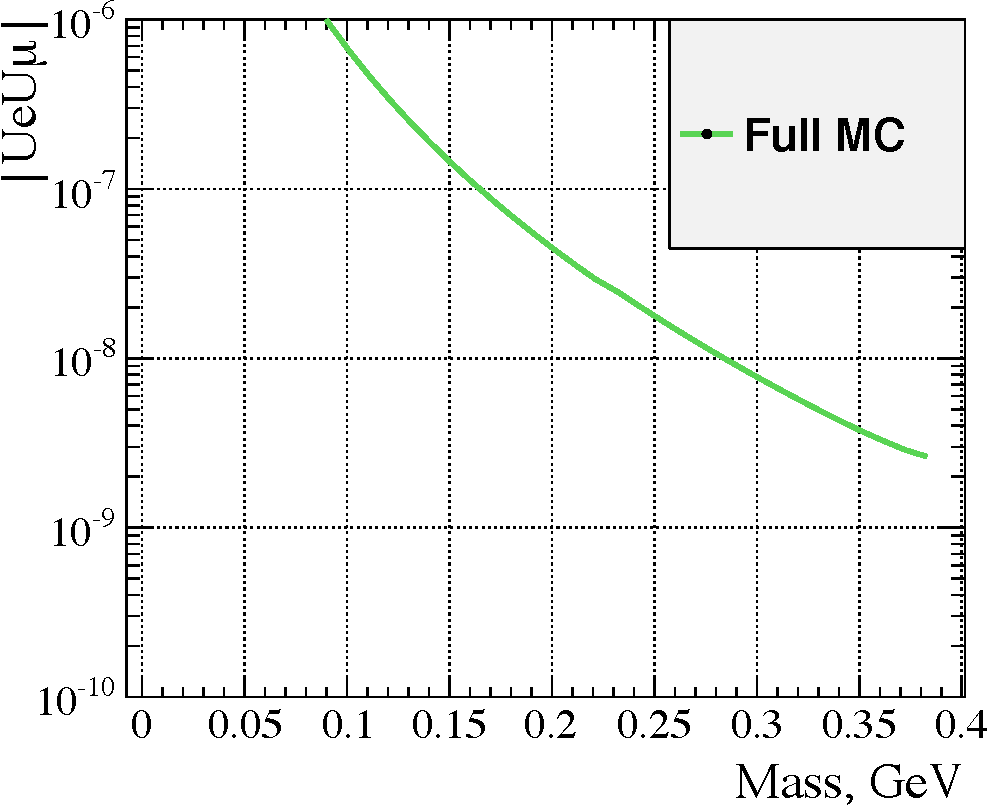
\includegraphics[width=\linewidth]{UmuUeThreeBody}  \\ a) $K\to\mu N\to \mu(ee\nu_e)$}
    \end{minipage}
    \hfill
    \begin{minipage}[!ht]{0.49\linewidth}
        \center{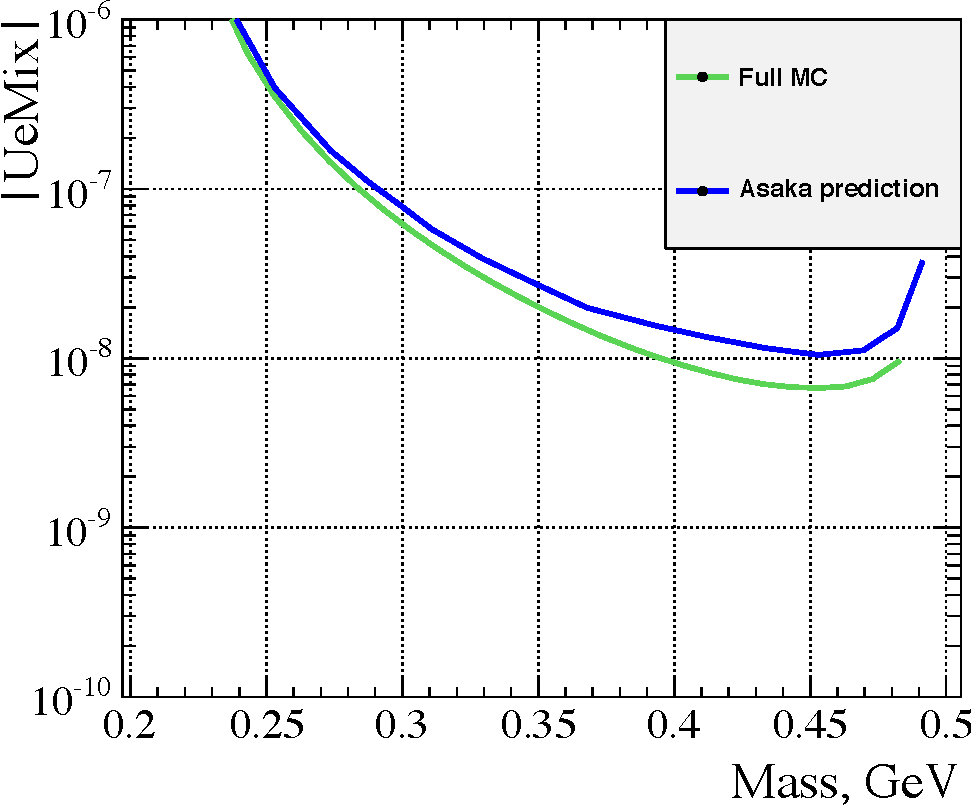
\includegraphics[width=\linewidth]{UeMixThreeBody} \\ b) $K\to eN\to e(\mu\mu\nu_{\mu,\tau})$}
    \end{minipage}
    \caption{Sensitivity of T2K to mixing elements in tree body decay modes: (a) for $\left|UeU\mu\right|$ and (b) for $\left|U_{e}\right|\sqrt{\left|U_{e}\right|^2+\left|U_{\tau}\right|^2}$. The detection efficiency of 100\% and no background are assumed.}
    \label{fig:HNL:ThreeBodySecond}
\end{figure}

An important 3-body mode is $K^+\rightarrow e(\mu^-\mu^+\nu_{e,\mu,\tau})$ because $\ell\bar{\ell}$ pairs can be produced together with any kind of the active neutrino due to  the NC process ~\cite{Johnson1997}. The mixing element for this process looks like $\left|U_{e}\right|\sqrt{\left|U_{e}\right|^2+\left|U_{\mu}\right|^2+\left|U_{\tau}\right|^2}$. Assuming $\left|U_e\right|^2 \gg\left|U_{\mu}\right|^2$, we can get some constraints on $\left|U_{e}\right|\sqrt{\left|U_{e}\right|^2+\left|U_{\tau}\right|^2}$ that wasn't obtained before in PS191 and limits on $\left|U_{\tau}\right|$ are also rather poor. Results for this decay mode are shown in Fig. ~\ref{fig:HNL:ThreeBodySecond} b.

As one can see, all our results are close to the estimation made by Asaka et al.

\subsection{HNL daughter particles}
Now we have information on the HNLs that enter ND280 and we generate their decays by using ROOT class TGenPhaseSpace. The decay points are randomly generated along the  HNL tracks inside the TPC volume. So the decay positions are expected to be uniformly distributed in this volume. Cross-check (Fig.~\ref{fig:HNL:decayPos}) shows some deviations at the upper and bottom edges for the large HNL mass but it was also expected due to the off-axis flux.

\begin{figure}[!ht]
    \center{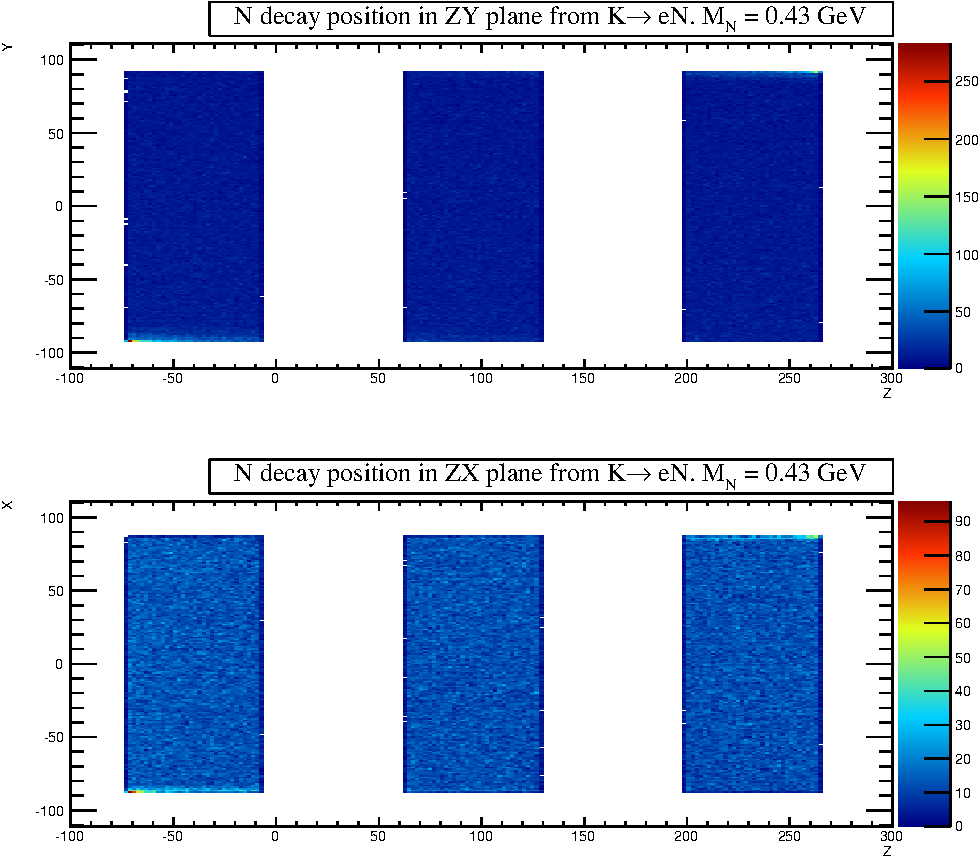
\includegraphics[width=0.7\linewidth]{DecayPos}}
    \caption{Distribution of HNL decay positions over 3 TPCs. The decay position is in the detector coordinate system in mm.}
    \label{fig:HNL:decayPos}
\end{figure}

Parameters of daughter particles are stored in the  nRooTracker tree for further work with nd280mc package. The weight of each HNL decay event is calculated as
\begin{equation}
    weight_{2-body}=weight_{K\rightarrow \ell N}\cdot\frac{L}{\beta\gamma c}\cdot\Gamma_{2-body},
\end{equation}
\begin{equation}
    weight_{3-body}=weight_{K\rightarrow \ell N}\cdot\frac{L}{\beta\gamma c}\cdot\cfrac{\cfrac{d\Gamma(p_1,p_2)}{dp_1dp_2}}{max\left(\cfrac{d\Gamma(p_1,p_2)}{dp_1dp_2}\right)}\cdot P,
\end{equation}
where $L$ is total length of HNL path in three TPCs and $P$ is a kinematic weight of the decay of the HNL, generated by TGenPhaseSpace.

After simulation of the HNL decays we have all information about kinematics of their daughter particles, i.e. momentum, direction, opening angles. This characteristics are presented in Fig.~\ref{fig:HNL:secondaryE}~and~\ref{fig:HNL:secondaryCos}. It's important to note that most of the particles have momentum below 2 GeV. Our TPCs was designed to reconstruct events in this energy region.
\begin{figure}[!ht]
\begin{center}
    \center{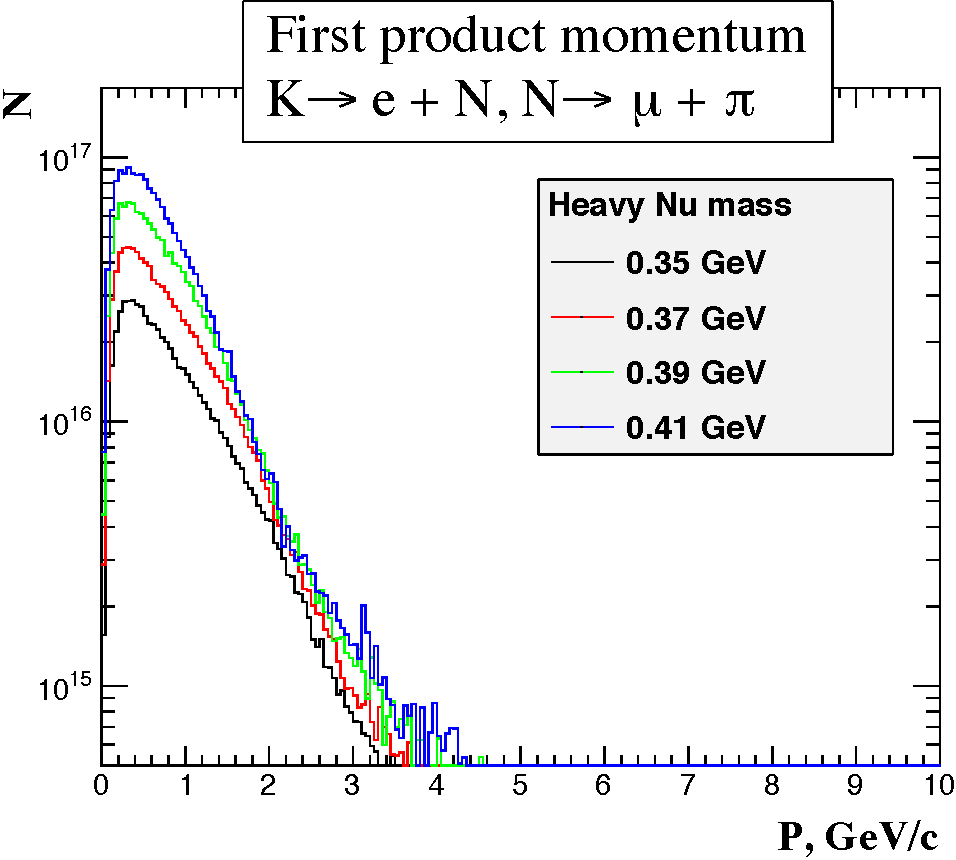
\includegraphics[width=0.8\linewidth]{SecMom}}
    \caption{Energy spectra of HNL daughter particles.}
    \label{fig:HNL:secondaryE}
\end{center}
\end{figure}
\begin{figure}[!ht]
\begin{center}
    \center{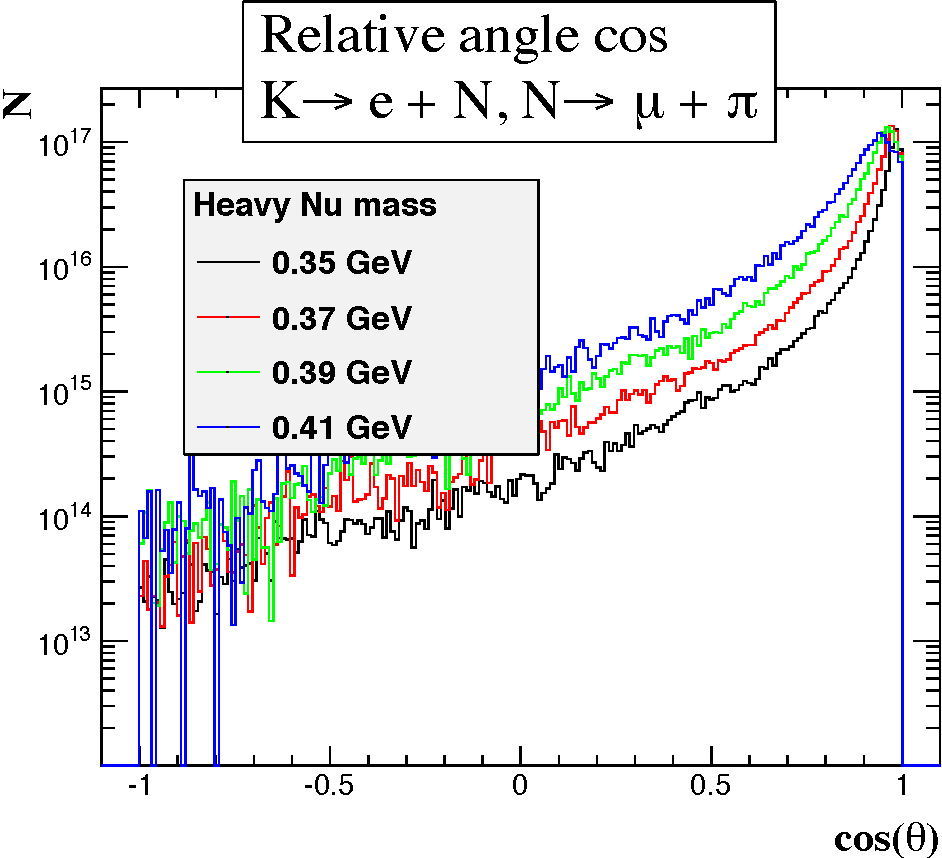
\includegraphics[width=0.8\linewidth]{SecRel}}
    \caption{Opening angle spectra of HNL daughter particles.}
    \label{fig:HNL:secondaryCos}
\end{center}
\end{figure}
The example of a ``good'' MC event with the HNL decay in the first TPC and further evolution of a daughter muon and a pion is shown in Fig.\ref{fig:HNL:event}
\begin{figure}[!ht]
   \center{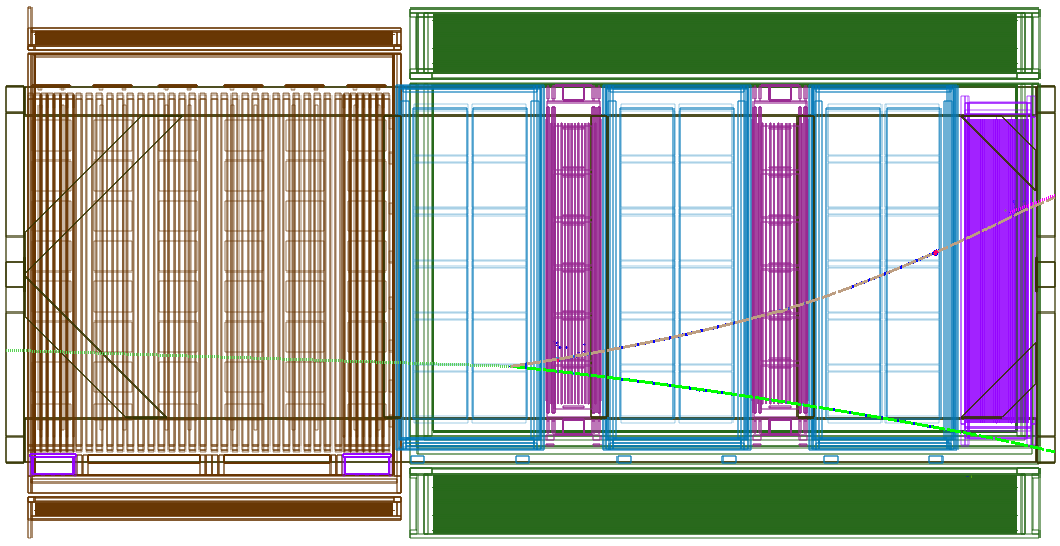
\includegraphics[width=0.8\linewidth]{goodeventMC}}
    \caption{Example of simulated event from HNL decay in the first TPC. Dashed green line corresponds to HNL track, green line to the muon track, brown line to the pion track.}
    \label{fig:HNL:event}
\end{figure}

\begin{comment}


\end{comment}


\chapter{Analysis}
\label{ch:HNL:ana}

\section{Time of flight correction}
\label{sec:HNL:tof_corr}
\section{Event selection}
\label{sec:HNL:sel}
\subsection{Signal event selection}
\subsection{Background suppression}
\label{sec:HNL:bg}

\section{Systematic uncertainties}
\subsection{Detector systematics}
\subsection{Flux systematics}
\subsection{Pile up}

\section{Statistical methods}
\label{sec:HNL:stat}


\chapter{Results}
\section{MC sensitivity estimations}

\section{Data unblinding}

\section{Prospects}
\end{document}